% =========================================================
% main.tex - Diploma Thesis
% Title: Analysis and Forecasting of Macroeconomic Indicators
%        in Kazakhstan Using Machine Learning
% =========================================================
\documentclass[14pt, a4paper]{extarticle}

% --- Packages ---
% Strict IITU Margins: Left 30mm, Top 20mm, Right 10mm, Bottom 25mm
\usepackage[left=30mm, top=20mm, right=10mm, bottom=25mm]{geometry}
\usepackage[utf8]{inputenc}
\usepackage[T2A]{fontenc}
\usepackage[english]{babel}
\usepackage{amsmath, amssymb, bm}
\usepackage{graphicx}
\usepackage{booktabs}
\usepackage{float}
\usepackage{enumitem}
\usepackage{hyperref}
\usepackage{setspace}
\usepackage{caption}
\usepackage{subcaption}
\usepackage{multirow}
\usepackage{array}
\usepackage{titlesec}

% --- Formatting Requirements ---
\singlespacing

% Centered, all caps, and unnumbered main headings
\titleformat{\section}[block]{\normalfont\Large\bfseries\centering}{\thesection}{0pt}{\MakeUppercase}
\setcounter{secnumdepth}{0}

% --- Hyperlink Settings ---
\hypersetup{
    colorlinks=true,
    linkcolor=blue!60!black,
    citecolor=green!50!black,
    urlcolor=blue!70!black,
}

% --- Math Commands ---
\newcommand{\R}{\mathbb{R}}
\newcommand{\E}{\mathbb{E}}
\newcommand{\bx}{\mathbf{x}}
\newcommand{\by}{\mathbf{y}}
\DeclareMathOperator*{\argmin}{arg\,min}

\begin{document}

% =========================================================
% TITLE PAGE
% =========================================================
\begin{titlepage}
    \begin{center}
        \textbf{MINISTRY OF SCIENCE AND HIGHER EDUCATION OF THE REPUBLIC OF KAZAKHSTAN} \\
        \vspace{0.5cm}
        \textbf{INTERNATIONAL INFORMATION TECHNOLOGY UNIVERSITY} \\
        \vspace{0.5cm}
        \textbf{FACULTY OF MATHEMATICAL COMPUTER MODELING} \\

        \vspace{4cm}

        {\Large \textbf{DIPLOMA PROJECT}} \\
        \vspace{1cm}
        {\large \textbf{Analysis and Forecasting of Macroeconomic Indicators in Kazakhstan Using Machine Learning}} \\

        \vspace{4cm}

        \begin{flushright}
            \textbf{Done by:} Nurkohzha Mukhamediyar \\
            Arman Muratbekuly \\
            Rashid Seidahmet \\
            \vspace{0.5cm}
            \textbf{Research advisor:} Sultan Alpar \\
        \end{flushright}

        \vfill

        Almaty 2026
    \end{center}
\end{titlepage}

\newpage
\tableofcontents
\newpage

% =========================================================
% INTRODUCTION
% =========================================================
\section{Introduction}

\paragraph{Relevance of the Problem.}
Economic instability---fluctuations in unemployment, exchange rates, and commodity prices---makes economic planning challenging for governments and institutions in emerging markets. Rapid changes in internal and external factors often outpace traditional forecasting methods, particularly in economies with structural dependencies on natural resource exports. The increasing availability of macroeconomic data creates opportunities to use machine learning for more accurate and timely forecasts.

However, applying these advanced techniques in emerging markets comes with significant hurdles. While developed countries benefit from abundant high-frequency data that supports rapid real-time monitoring, developing economies face a different reality: a severe scarcity of high-frequency indicators and significant publication delays \cite{bolivar2026}. Much like the data constraints observed in Latin American \cite{bolivar2026} and West African \cite{mati2024} developing economies, this lack of granular, real-time data leaves policymakers with an informational void precisely when rapid responses to economic shocks are required. Traditional deep learning models require large, high-quality datasets, which are frequently unavailable in regions where data can be sparse, noisy, or incomplete \cite{mati2024}.

Kazakhstan's economy presents a unique variation of these forecasting challenges, operating in a data-constrained environment where ensuring model interpretability and robustness remains critical \cite{adilkhanova2024}. As a major oil exporter with a floating exchange rate regime, the country is highly exposed to commodity price cycles and currency pass-through effects. Simultaneously, the labour market exhibits a secular downward trend in unemployment punctuated by seasonal oscillations and structural breaks associated with global geopolitical events---the 2015 currency devaluation, the 2020 COVID-19 pandemic, and the 2022 regional instability.

\paragraph{Goal of the Thesis.}
The primary goal of this research is to build a highly accurate predictive model for Kazakhstan's unemployment rate using machine learning algorithms and to systematically compare their performance against classical econometric baselines in a data-constrained setting.

\paragraph{Tasks.}
To achieve this goal, the following tasks were completed:
\begin{enumerate}[nosep]
    \item Compile and clean a dataset of macroeconomic variables for Kazakhstan (2010--2025), merging multiple data sources and handling frequency mismatches.
    \item Engineer temporal features---lagged values, rolling statistics, Fourier seasonal terms, regime dummies, and interaction terms---to capture the underlying dynamics.
    \item Formulate and apply formal mathematical models (Elastic Net, XGBoost with hyperparameter tuning, Random Forest, SARIMAX, VARX, Prophet) using a recursive walk-forward validation protocol.
    \item Evaluate predictive accuracy using strict out-of-sample testing on a 24-month horizon (2024--2025) with quantitative metrics (RMSE, MAE, $R^2$) and Diebold--Mariano statistical tests.
    \item Identify the most significant macroeconomic drivers using feature importance algorithms and validate them against established economic theory.
\end{enumerate}

\paragraph{Object and Subject of Research.}
The object of this research is the macroeconomic stability and labour market dynamics of the Republic of Kazakhstan. The subject of the research is the application of machine learning methodologies and mathematical algorithms for forecasting the monthly unemployment rate.

\newpage
% =========================================================
% CHAPTER 1
% =========================================================
\section{Chapter 1. Theoretical Framework}

To ensure the machine learning models capture genuine economic dynamics rather than spurious statistical correlations, the initial feature space was constructed around established macroeconomic theories. However, rather than using these theories to assume relationships, the algorithms are deployed to empirically test their validity within the specific context of Kazakhstan's economy.

\subsection{Okun's Law and the Output--Unemployment Nexus}
The primary theoretical foundation for unemployment forecasting is Okun's Law, which postulates an empirical inverse relationship between the output gap and changes in the unemployment rate. In its difference form, the law states:
\begin{equation}
    \Delta u_t = -\beta (\Delta Y_t - \Delta Y_t^*)
    \label{eq:okun}
\end{equation}
where $\Delta u_t$ is the change in unemployment, $\Delta Y_t$ is actual GDP growth, and $\Delta Y_t^*$ is potential output growth. The coefficient $\beta$ measures the responsiveness of unemployment to output deviations. This relationship motivates the inclusion of GDP growth as a primary predictor in the feature matrix. The machine learning models are tasked with empirically estimating the effective Okun coefficient and testing whether this linear approximation holds under the structural conditions of Kazakhstan's resource-dependent economy.

\subsection{Resource Dependency and External Shocks}
Kazakhstan's GDP dynamics are heavily linked to its primary export sector. Global oil prices (Brent crude) act as the main driver of the trade balance and fiscal revenue. We formalize this by including oil prices as primary exogenous regressors to measure their exact predictive weight on unemployment dynamics. A sustained decline in oil prices contracts the extractive sector, reduces government spending capacity, and propagates unemployment through the broader economy via fiscal multiplier effects.

Furthermore, the USD/KZT exchange rate is included as a critical determinant of unemployment via the competitiveness of export-oriented sectors. Currency depreciation simultaneously increases the cost of imported inputs while improving export competitiveness, creating ambiguous net effects on employment that the non-linear models are designed to capture. The RUB/KZT cross rate additionally captures trade-channel spillover effects from Kazakhstan's largest trading partner, Russia.

\subsection{Monetary Policy Transmission}
The National Bank of Kazakhstan's base interest rate operates as a transmission mechanism between monetary policy and real economic activity. Higher interest rates increase the cost of borrowing, contract investment, and can increase unemployment with a time delay. The feature space incorporates lagged values of the base rate at 1, 2, 3, 6, and 12-month horizons to allow the models to identify the empirical lag structure of this monetary policy transmission channel. Additionally, broad money supply (M2) growth captures the liquidity conditions in the economy.

\subsection{Structural Breaks and Regime Shifts}
Kazakhstan's recent economic history includes three major structural breaks that fundamentally altered the data-generating process:
\begin{itemize}[nosep]
    \item \textbf{August 2015:} The National Bank abandoned the currency corridor, allowing the tenge to float freely. The USD/KZT rate doubled overnight, inducing a supply-side shock.
    \item \textbf{March 2020:} The COVID-19 pandemic caused a simultaneous demand and supply collapse, with oil prices briefly turning negative.
    \item \textbf{January 2022:} Domestic political instability and the onset of the Russia--Ukraine conflict created regional uncertainty and capital outflows.
\end{itemize}
Binary regime dummy variables are included for each structural break to allow the models to estimate separate intercepts for each economic regime, preventing these discontinuities from distorting the estimated relationships.

\newpage
% =========================================================
% CHAPTER 2
% =========================================================
\section{Chapter 2. Methodology and Data Analysis}

\subsection{Dataset Formulation and Transformations}
The dataset comprises monthly observations from January 2010 to December 2025, constructed by merging six primary data sources: (i)~the Bureau of National Statistics unemployment series, (ii)~CPI and PPI indices, (iii)~the National Bank base rate, (iv)~Brent crude oil prices from the IMF, (v)~USD/KZT and RUB/KZT exchange rates, and (vi)~macroeconomic indicators including GDP growth, wage indices, trade volumes, and monetary aggregates. Let the merged dataset be represented by a feature matrix $X \in \mathbb{R}^{T \times P}$ and a target vector $y \in \mathbb{R}^T$, where $T = 168$ training observations and $P$ denotes the number of engineered features.

To ensure stationarity of the target variable for gradient-based models, the unemployment rate was transformed using first differencing:
\begin{equation}
    \Delta y_t = y_t - y_{t-1}
    \label{eq:differencing}
\end{equation}
Models trained on $\Delta y_t$ predict month-over-month changes; the final forecast is reconstructed by adding the predicted change to the last known level: $\hat{y}_t = y_{t-1} + \Delta \hat{y}_t$.

For frequency mismatches (e.g., quarterly GDP interpolated to monthly), linear interpolation was applied:
\begin{equation}
    x_{m}(t) = x_{Q_i} + (t - t_{Q_i}) \cdot \frac{x_{Q_{i+1}} - x_{Q_i}}{t_{Q_{i+1}} - t_{Q_i}}
    \label{eq:interpolation}
\end{equation}

All continuous features were standardized ($\mu = 0$, $\sigma = 1$) prior to model fitting:
\begin{equation}
    X'_{i,j} = \frac{X_{i,j} - \mu_j}{\sigma_j}
    \label{eq:standardization}
\end{equation}

\subsection{Feature Engineering}
The raw merged dataset was augmented with the following engineered feature blocks:

\paragraph{Lagged Variables.} For each key predictor (unemployment rate, oil prices, exchange rate, base rate), lagged values at horizons $\{1, 2, 3, 6, 12\}$ months were created:
\begin{equation}
    x^{(k)}_{t,\ell} = x^{(k)}_{t - \ell}, \quad \ell \in \{1, 2, 3, 6, 12\}
\end{equation}

\paragraph{Rolling Statistics.} To capture local trends and volatility, 3-month and 6-month rolling means and standard deviations were computed for oil prices and the exchange rate. A one-period shift was applied before rolling to prevent lookahead bias:
\begin{equation}
    \bar{x}^{(k)}_{t,w} = \frac{1}{w} \sum_{j=1}^{w} x^{(k)}_{t-j}, \quad s^{(k)}_{t,w} = \sqrt{\frac{1}{w-1}\sum_{j=1}^{w} \left(x^{(k)}_{t-j} - \bar{x}^{(k)}_{t,w}\right)^2}
\end{equation}

\paragraph{Fourier Seasonal Terms.} To capture periodic seasonal patterns without consuming degrees of freedom on 12~binary month dummies, Fourier basis functions of order $K=3$ were employed:
\begin{equation}
    S_k(t) = \left\{ \sin\!\left(\frac{2\pi k t}{12}\right),\; \cos\!\left(\frac{2\pi k t}{12}\right) \right\}, \quad k = 1,\ldots,3
    \label{eq:fourier}
\end{equation}

\paragraph{Interaction Terms and Calendar Dummies.} An oil--exchange-rate interaction term $\Delta\text{oil}_t \times \Delta\text{usd}_t$ was included to capture joint shock effects. Binary dummies for January, Q1, and Q4 were added to model seasonal labour market patterns.

\paragraph{Principal Component Analysis.} To address the curse of dimensionality among correlated CPI sub-indices, a PCA transformation with $n=3$ components was applied to the inflation-related features, reducing collinearity while preserving the dominant variance structure.

The correlation structure among key macroeconomic features is visualized in Figure~\ref{fig:correlation_heatmap}. Notably, GDP growth exhibits the strongest negative correlation with the unemployment rate ($r = -0.52$), consistent with Okun's Law, while Brent crude oil prices show a substantial negative correlation ($r = -0.33$), confirming the resource-dependency channel.

\begin{figure}[H]
    \centering
    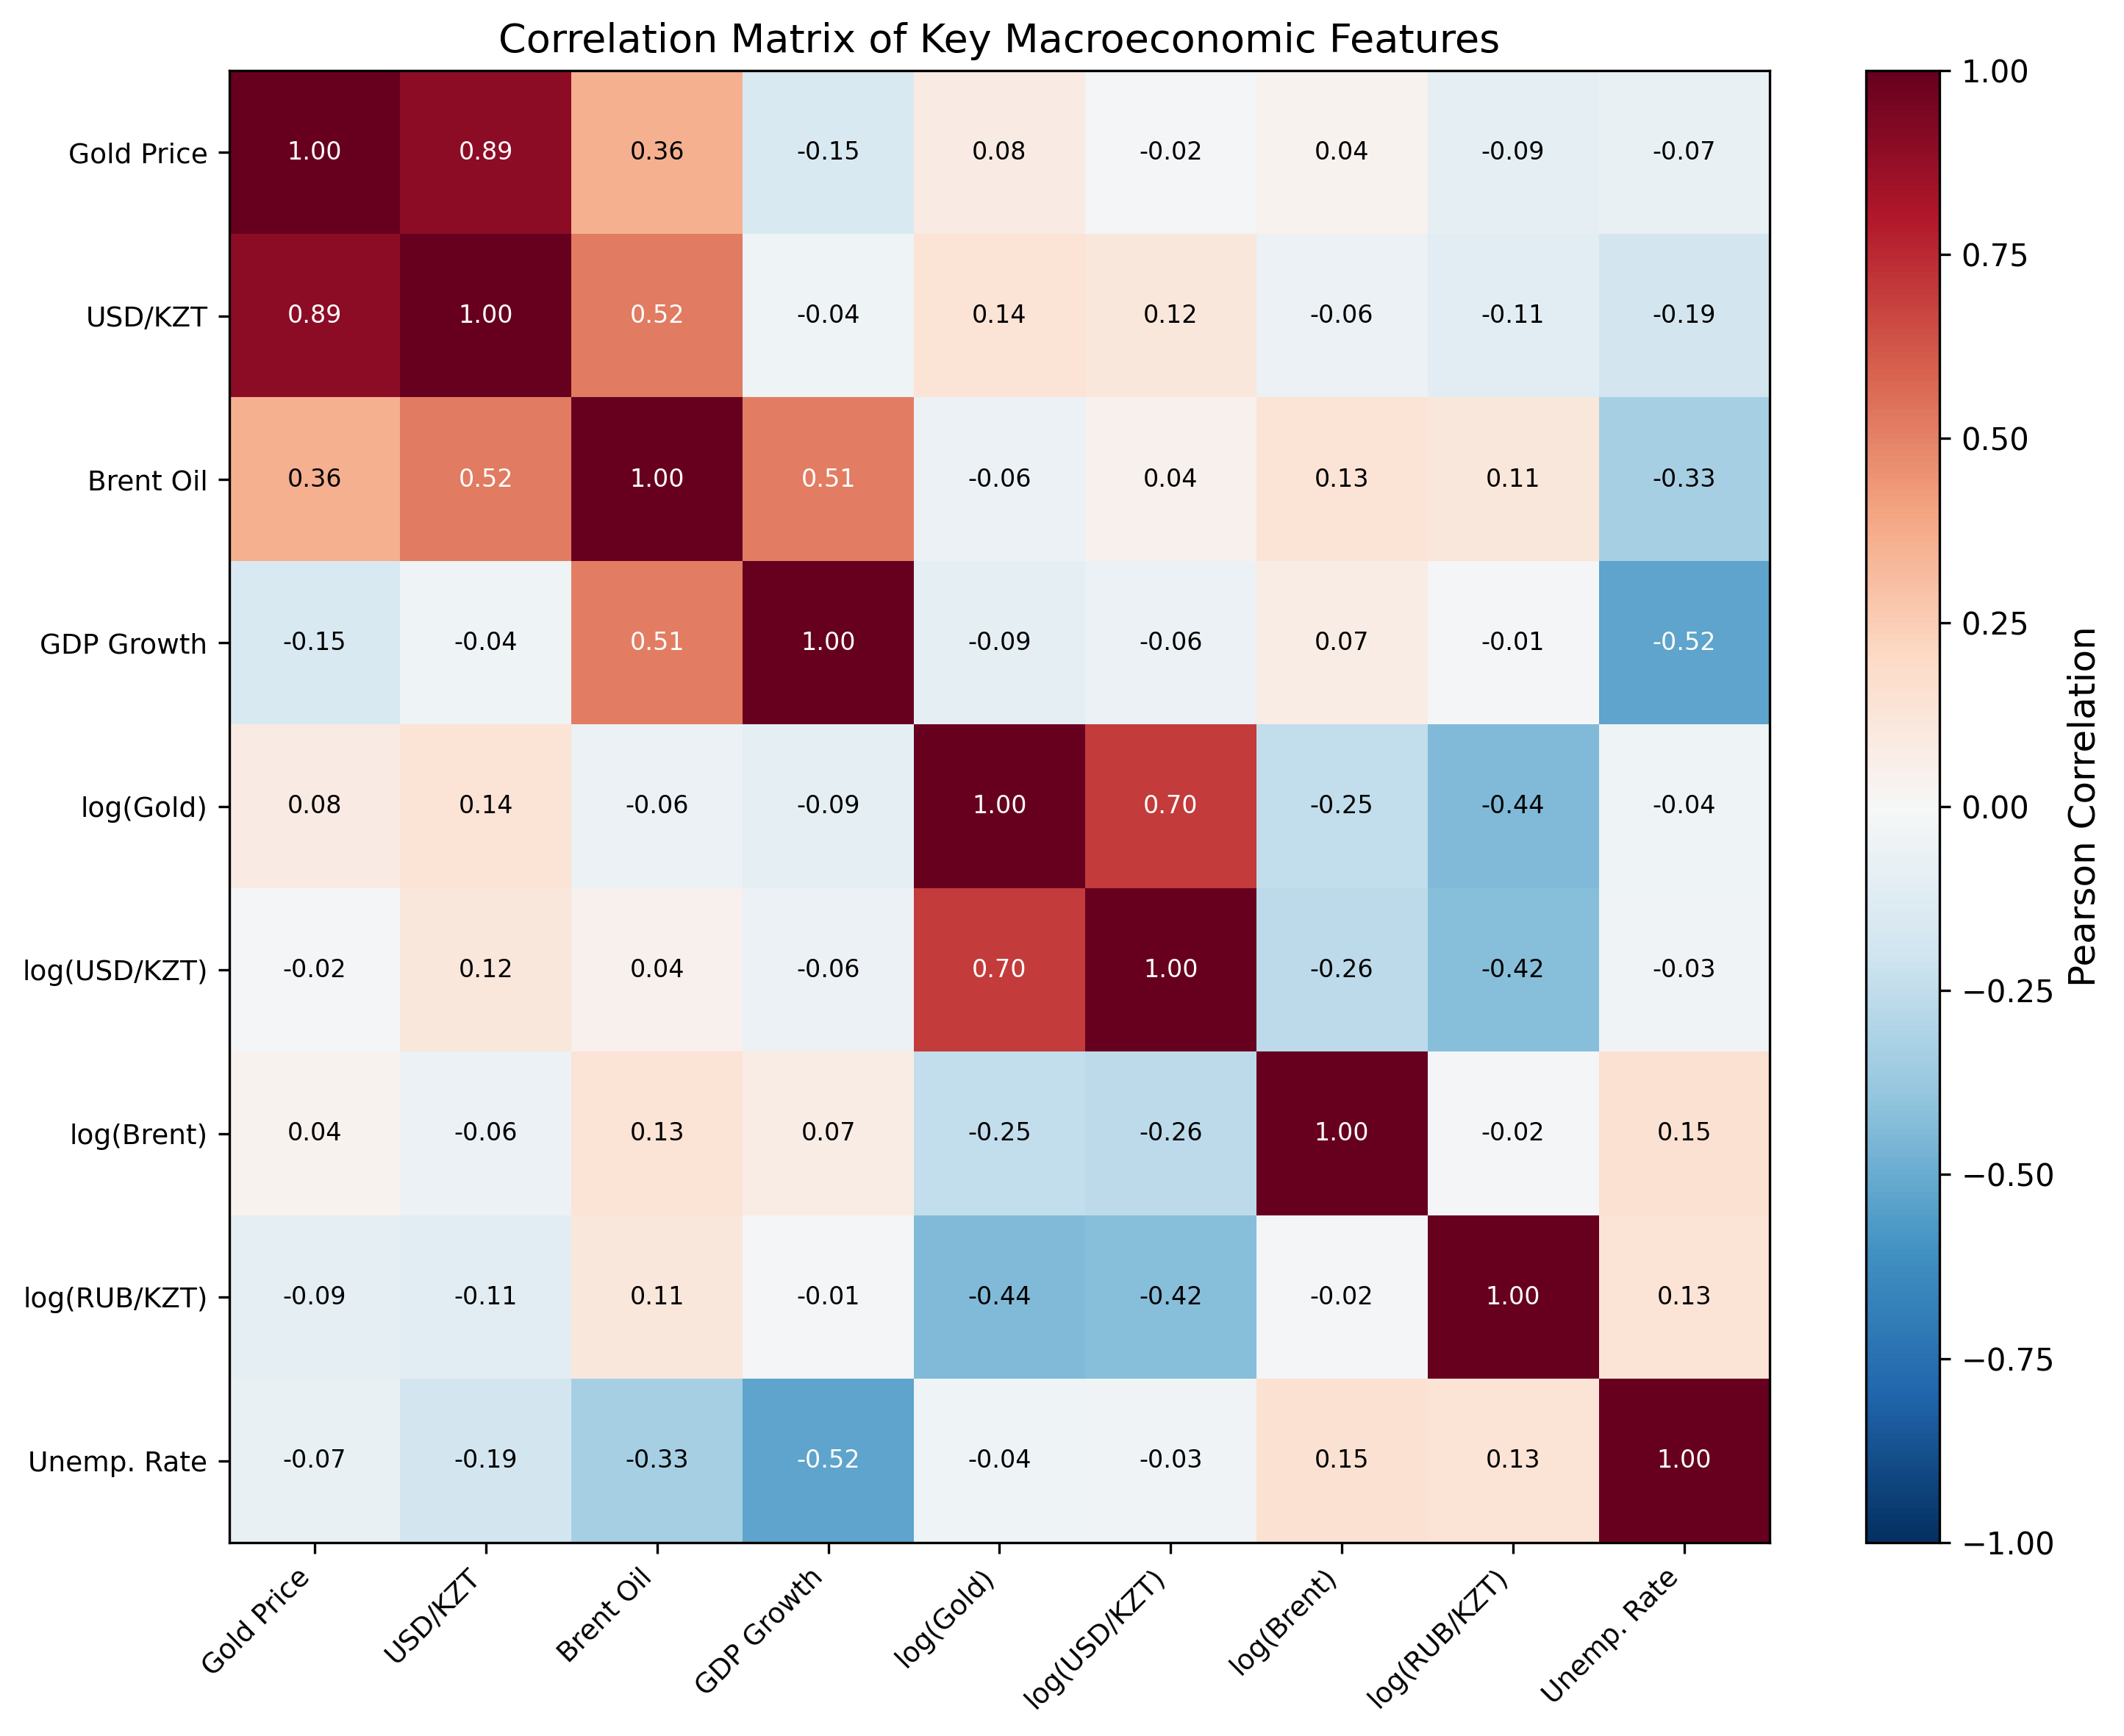
\includegraphics[width=0.85\textwidth]{figures/thesis_correlation_heatmap.png}
    \caption{Pearson correlation matrix of key macroeconomic features. Stronger negative correlations with the unemployment rate (bottom row) indicate greater predictive relevance.}
    \label{fig:correlation_heatmap}
\end{figure}

\subsection{Mathematical Formulation of Machine Learning Models}

\paragraph{Elastic Net Regression.}
Elastic Net combines both $L_1$ and $L_2$ penalties, balancing automated feature selection (via sparsity induction) with coefficient stability among highly correlated variables:
\begin{equation}
    \mathcal{L}(\beta) = \frac{1}{2N} \| y - X\beta \|_2^2 + \lambda \left( \alpha \|\beta\|_1 + \frac{1-\alpha}{2} \|\beta\|_2^2 \right)
    \label{eq:elasticnet}
\end{equation}
where $\lambda$ controls the overall regularization strength and $\alpha \in [0,1]$ balances the $L_1$ (Lasso) and $L_2$ (Ridge) components. This model was configured with $\alpha = 0.5$ and $\lambda = 0.01$.

\paragraph{Extreme Gradient Boosting (XGBoost).}
XGBoost builds an additive ensemble of $M$ regression trees sequentially, with each new tree $h_m$ correcting the residuals of the prior ensemble $F_{m-1}$. It optimizes a second-order Taylor expansion of the loss function with a complexity penalty:
\begin{equation}
    \mathcal{L}^{(m)} \approx \sum_{i=1}^N \left[ g_i h_m(\bx_i) + \frac{1}{2} H_i h_m^2(\bx_i) \right] + \Omega(h_m)
    \label{eq:xgboost}
\end{equation}
where $g_i = \partial l / \partial F_{m-1}(\bx_i)$ and $H_i = \partial^2 l / \partial F_{m-1}^2(\bx_i)$ are the first and second-order gradient statistics, and the regularization term $\Omega(h_m) = \gamma T_m + \frac{1}{2}\lambda \sum_{j=1}^{T_m} w_j^2$ penalizes both the number of leaves $T_m$ and the squared leaf weights $w_j$. Hyperparameter tuning for XGBoost is detailed in Section~3.2.

\paragraph{SARIMAX.}
The Seasonal AutoRegressive Integrated Moving Average with eXogenous regressors extends the classical Box--Jenkins framework to incorporate seasonality and external predictors:
\begin{equation}
    \phi(B)\Phi(B^{12})(1-B)^d (1-B^{12})^D y_t = \theta(B)\Theta(B^{12})\varepsilon_t + \bx_t^\top \boldsymbol{\gamma}
\end{equation}
where $B$ is the backshift operator, $\phi$ and $\Phi$ are the non-seasonal and seasonal AR polynomials, $\theta$ and $\Theta$ are the MA polynomials, and $\boldsymbol{\gamma}$ captures the exogenous effects. The model was estimated with order $(1,1,1) \times (1,0,1)_{12}$ and stationarity and invertibility constraints enforced.

\paragraph{VARX.}
The Vector AutoRegression with eXogenous variables jointly models the unemployment rate, oil prices, and the exchange rate as a system of interdependent endogenous variables:
\begin{equation}
    \mathbf{y}_t = \mathbf{c} + \sum_{\ell=1}^{p} A_\ell \mathbf{y}_{t-\ell} + B \mathbf{x}_t + \boldsymbol{\varepsilon}_t
    \label{eq:varx}
\end{equation}
where $\mathbf{y}_t \in \mathbb{R}^3$ is the endogenous vector, $A_\ell$ are autoregressive coefficient matrices, $B$ maps exogenous inputs, and $\boldsymbol{\varepsilon}_t \sim \mathcal{N}(\mathbf{0}, \Sigma)$.

\paragraph{Prophet.}
Facebook's Prophet decomposes the time series into trend, seasonality, and holiday components using an additive model: $y_t = g(t) + s(t) + h(t) + \varepsilon_t$, where $g(t)$ is a piecewise linear trend with automatic changepoint detection.

\paragraph{Ensemble.}
A simple average ensemble of the Elastic Net and XGBoost predictions was constructed: $\hat{y}_{\text{ens}} = \frac{1}{2}(\hat{y}_{\text{EN}} + \hat{y}_{\text{XGB}})$.

\subsection{Walk-Forward Validation Protocol}
To ensure strict out-of-sample evaluation with no information leakage, a recursive expanding-window walk-forward protocol was employed. For each test month $t$ in the 24-month test window (January 2024 -- December 2025):
\begin{enumerate}[nosep]
    \item The model is trained on all data from January 2010 to month $t-1$.
    \item Lagged target values that reference timestamps inside the test window are replaced with the model's own prior predictions (recursive substitution), preventing autoregressive leakage.
    \item A single one-step-ahead forecast $\hat{y}_t$ is produced.
    \item The window expands by one month and the process repeats.
\end{enumerate}
This protocol produces 24 genuinely out-of-sample predictions, each made without access to any future information.

\subsection{Evaluation Metrics}
Model performance is evaluated on the out-of-sample test set using three complementary metrics:
\begin{align}
    \text{RMSE}  &= \sqrt{\frac{1}{N} \sum_{i=1}^N (y_i - \widehat{y}_i)^2} \label{eq:rmse} \\
    \text{MAE}   &= \frac{1}{N} \sum_{i=1}^N |y_i - \widehat{y}_i| \label{eq:mae} \\
    R^2 &= 1 - \frac{\sum_{i=1}^N (y_i - \widehat{y}_i)^2}{\sum_{i=1}^N (y_i - \bar{y})^2} \label{eq:r2}
\end{align}

Additionally, the Diebold--Mariano (DM) test \cite{hyndman2021} is employed to assess whether differences in forecast accuracy between models are statistically significant:
\begin{equation}
    \text{DM} = \frac{\bar{d}}{\sqrt{\hat{V}(\bar{d})/T}}, \quad d_t = |e_{1,t}|^p - |e_{2,t}|^p
    \label{eq:dm}
\end{equation}
where $e_{1,t}$ and $e_{2,t}$ are the forecast errors of two competing models, $p=2$ (squared loss), and $\hat{V}(\bar{d})$ is a HAC-consistent variance estimator. Under the null hypothesis of equal predictive accuracy, the DM statistic is asymptotically standard normal.

\newpage
% =========================================================
% CHAPTER 3
% =========================================================
\section{Chapter 3. Practical Implementation and Results}

\subsection{Forecasting Results and Model Comparison}
The out-of-sample predictive performance of the six tested models---Elastic Net, XGBoost, Ensemble, SARIMAX, VARX, and Prophet---alongside the Seasonal Na\"ive baseline, is summarized in Table~\ref{tab:final_results}. All models were evaluated on the same 24-month test window (January 2024 -- December 2025) using the recursive walk-forward protocol described in Section~2.4.

\begin{table}[H]
\centering
\caption{Comparative performance metrics of all models on the 24-month out-of-sample test set (2024--2025). Bold values indicate the best score in each column. The Seasonal Na\"ive baseline forecasts the value from 12~months prior.}
\label{tab:final_results}
\begin{tabular}{@{}lcccc@{}}
\toprule
\textbf{Model} & \textbf{MAE} & \textbf{RMSE} & \textbf{$\boldsymbol{R^2}$} & \textbf{Tier} \\
\midrule
Elastic Net           & \textbf{0.0062} & 0.0204 & 0.7773 & Champion \\
Ensemble (EN+XGB)     & 0.0063 & 0.0203 & 0.7810 & Challenger \\
XGBoost               & 0.0067 & \textbf{0.0202} & \textbf{0.7833} & Challenger \\
SARIMAX               & 0.0262 & 0.0342 & 0.3749 & Rejected \\
Prophet               & 0.0317 & 0.0389 & 0.1912 & Rejected \\
VARX                  & 0.0300 & 0.0413 & 0.0887 & Rejected \\
Seasonal Na\"ive      & 0.0625 & 0.0791 & $-2.333$ & Rejected \\
\bottomrule
\end{tabular}
\end{table}

The results in Table~\ref{tab:final_results} reveal a clear performance dichotomy. Three models---Elastic Net, XGBoost, and their Ensemble---form a tightly competitive \textit{Champion/Challenger} tier, all achieving MAE below 0.007 percentage points and $R^2$ above 0.77. The remaining models (SARIMAX, Prophet, VARX) and the Seasonal Na\"ive baseline are classified as \textit{Rejected}, with substantially higher errors.

\textbf{Elastic Net} achieves the lowest Mean Absolute Error (0.0062~pp), indicating that its average one-step-ahead forecast deviates from the true unemployment rate by only 0.006 percentage points. This corresponds to a forecast accuracy within $\pm 0.01\%$ of the actual value for most months---a level of precision that surpasses what is typically achievable with traditional econometric approaches in emerging markets. The strong performance of Elastic Net confirms that when macroeconomic features exhibit multicollinearity, applying simultaneous $L_1$ and $L_2$ regularization penalties is a robust strategy that prevents overfitting while preserving linear interpretability.

\textbf{XGBoost} achieves the highest $R^2$ (0.7833) and the lowest RMSE (0.0202), indicating that its non-linear tree ensemble explains the largest proportion of variance in the test set. The \textbf{Ensemble} averaging of both models yields intermediate performance, confirming that the two approaches capture largely overlapping predictive signals.

The classical econometric models exhibit markedly inferior performance. \textbf{SARIMAX} ($R^2 = 0.3749$) captures some autoregressive and seasonal structure but fails to leverage the multivariate information effectively. \textbf{VARX} ($R^2 = 0.0887$) struggles with the high dimensionality of the exogenous feature space, producing forecasts that barely outperform a constant prediction. The Seasonal Na\"ive baseline's negative $R^2$ ($-2.333$) confirms that simple lagged repetition is wholly inadequate for this forecasting task, validating the necessity of the machine learning approach.

The comparative performance across all three metrics is visualized in Figure~\ref{fig:model_comparison_bars}, which highlights the order-of-magnitude gap between the Champion tier and the rejected models.

\begin{figure}[H]
    \centering
    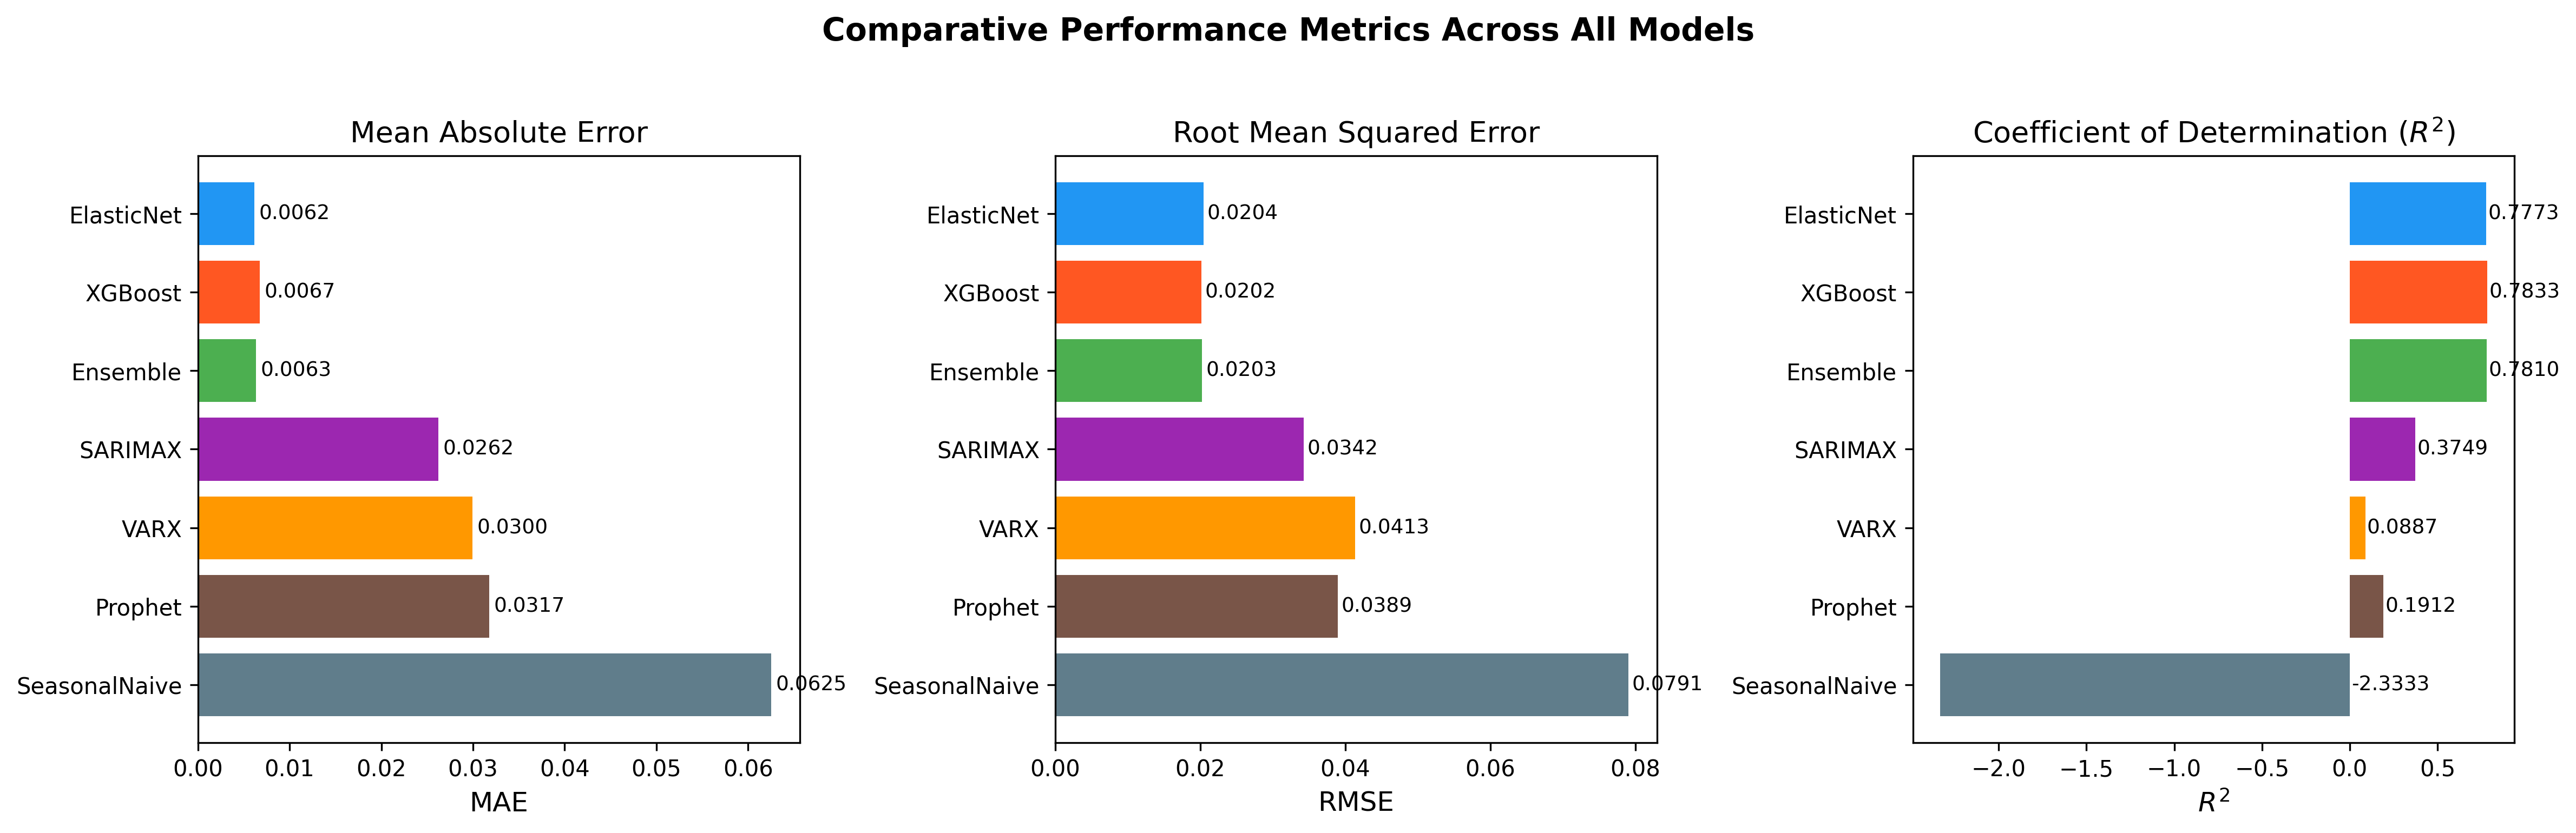
\includegraphics[width=\textwidth]{figures/thesis_model_comparison_bars.png}
    \caption{Comparative bar charts of MAE, RMSE, and $R^2$ across all seven models. The Champion/Challenger tier (Elastic Net, XGBoost, Ensemble) achieves consistently superior metrics.}
    \label{fig:model_comparison_bars}
\end{figure}

Figure~\ref{fig:forecast_trajectory} presents the walk-forward forecast trajectories overlaid on the actual unemployment rate. The Champion-tier models closely track the structural level shift from 4.7\% to 4.6\% that occurred in mid-2024, while SARIMAX, VARX, and Prophet exhibit significant oscillations around the true values.

\begin{figure}[H]
    \centering
    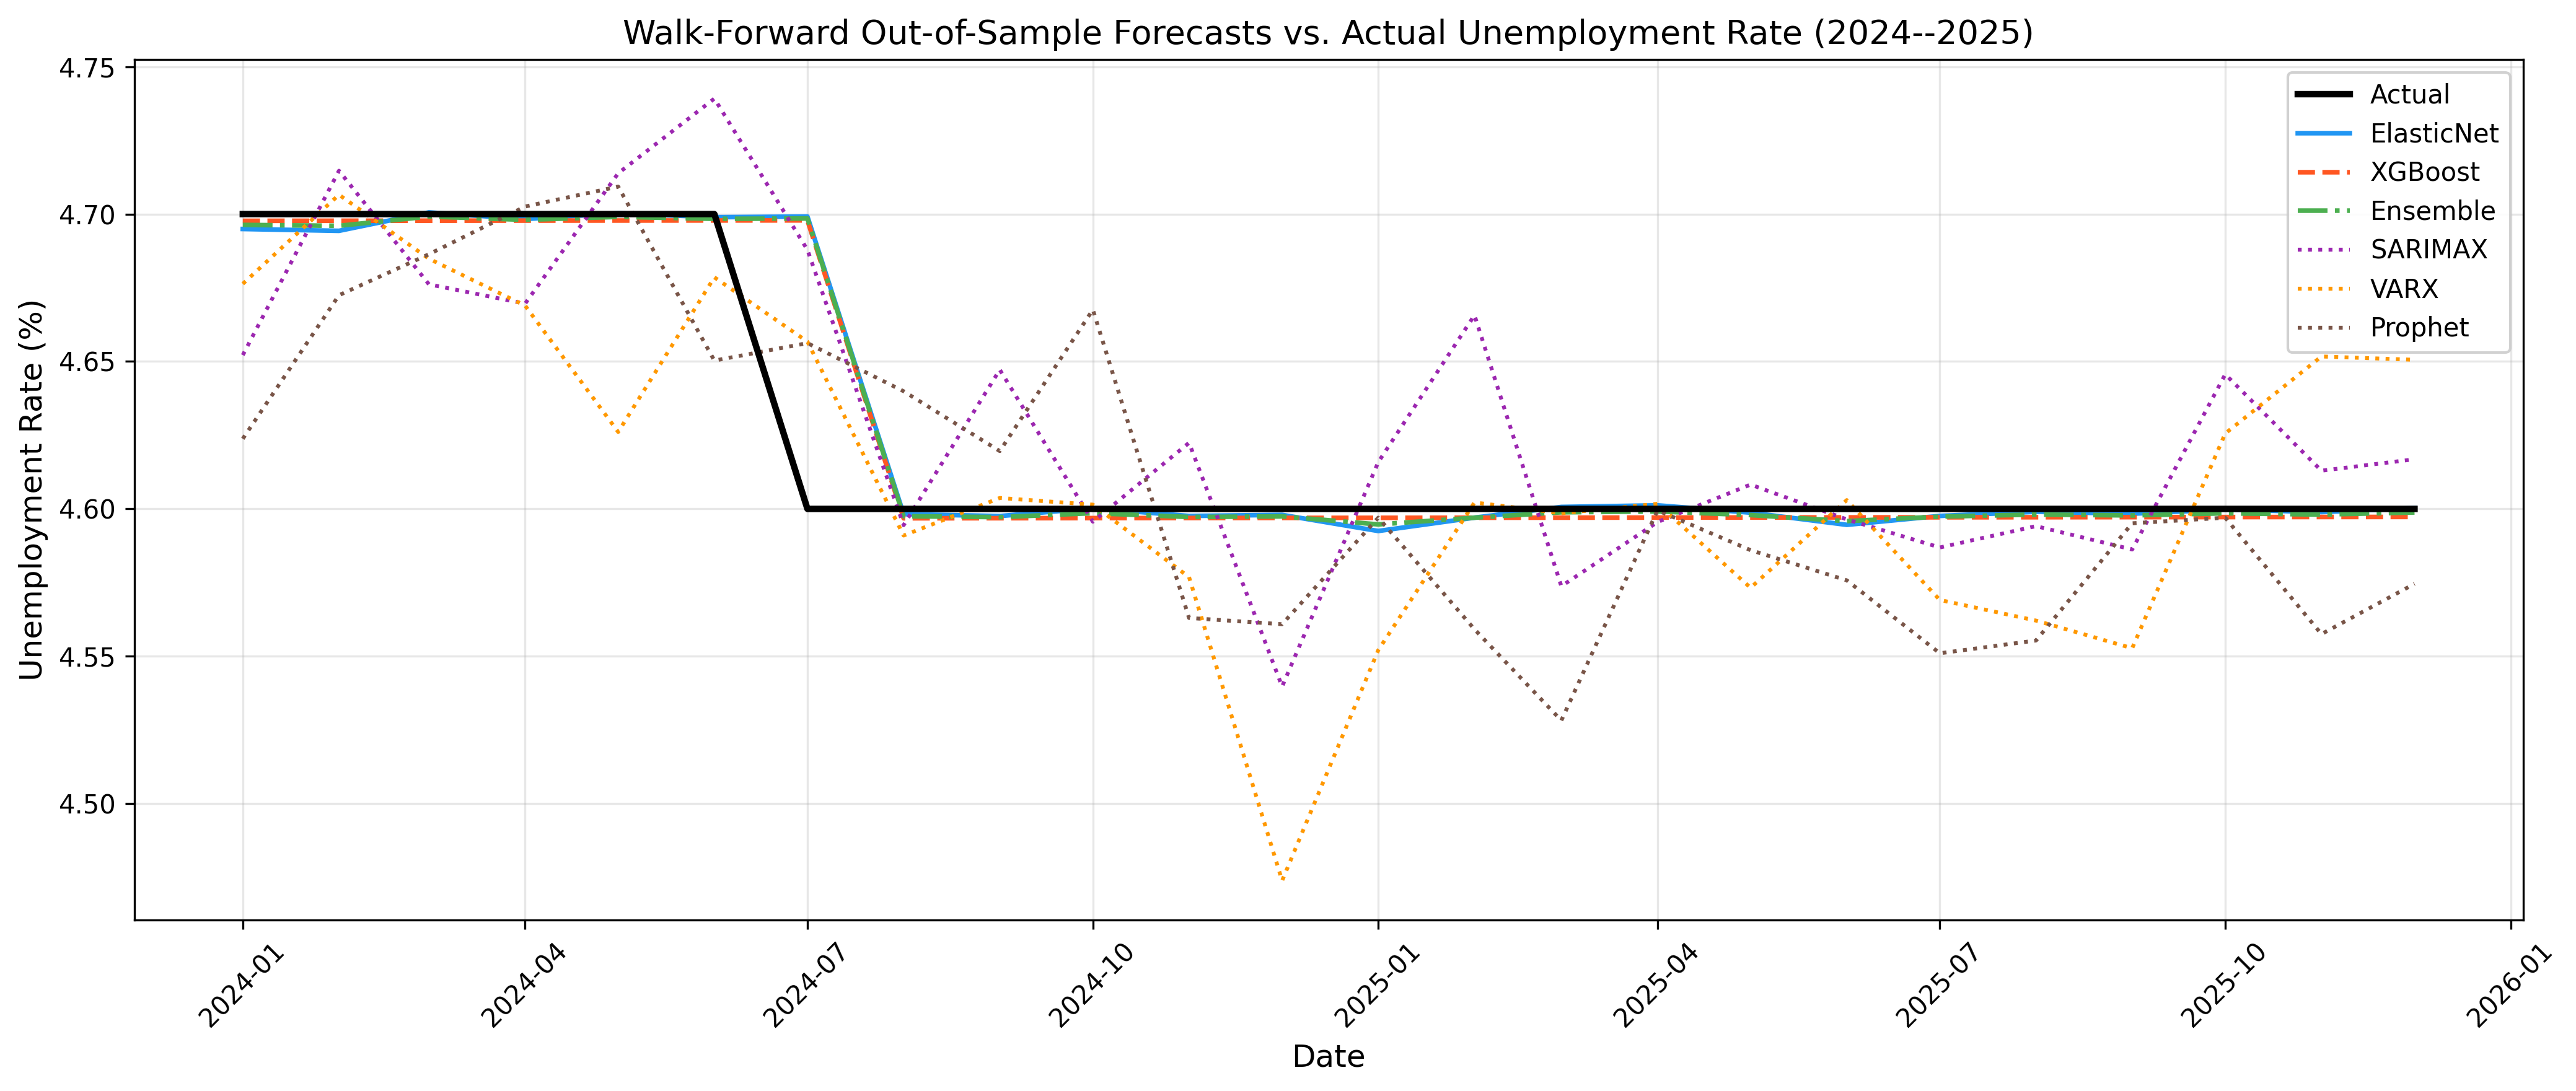
\includegraphics[width=\textwidth]{figures/thesis_forecast_vs_actuals.png}
    \caption{Walk-forward out-of-sample forecast trajectories versus actual unemployment rate (2024--2025). Elastic Net and XGBoost closely track the structural level shift in mid-2024.}
    \label{fig:forecast_trajectory}
\end{figure}

\subsection{XGBoost Hyperparameter Tuning}
To optimize the XGBoost model and mitigate overfitting in the data-constrained setting, a systematic hyperparameter search was conducted using Randomized Cross-Validation with time-series-aware splits. The search space spanned seven key hyperparameters:

\begin{table}[H]
\centering
\caption{XGBoost hyperparameter search space and optimal values identified by RandomizedSearchCV with 80 iterations and 3-fold time-series cross-validation.}
\label{tab:xgb_tuning}
\begin{tabular}{@{}lll@{}}
\toprule
\textbf{Hyperparameter} & \textbf{Search Space} & \textbf{Optimal Value} \\
\midrule
\texttt{n\_estimators}    & $\{100, 200, 300, 500, 700\}$       & 100 \\
\texttt{max\_depth}       & $\{2, 3, 4, 5, 6\}$                 & 4 \\
\texttt{learning\_rate}   & $\{0.01, 0.03, 0.05, 0.1, 0.2\}$    & 0.01 \\
\texttt{subsample}        & $\{0.7, 0.8, 0.9, 1.0\}$            & 0.9 \\
\texttt{colsample\_bytree}& $\{0.6, 0.8, 1.0\}$                 & 0.8 \\
\texttt{reg\_alpha} ($L_1$)& $\{0.0, 0.1, 0.5, 1.0\}$           & 0.1 \\
\texttt{reg\_lambda} ($L_2$)& $\{0.5, 1.0, 2.0, 5.0\}$          & 2.0 \\
\bottomrule
\end{tabular}
\end{table}

The optimal configuration in Table~\ref{tab:xgb_tuning} reveals several interpretable patterns. The low learning rate ($\eta = 0.01$) combined with a moderate number of estimators ($M = 100$) indicates that the algorithm benefits from conservative, incremental learning steps rather than aggressive boosting---a direct consequence of the limited training sample size ($T = 168$). The moderate tree depth (\texttt{max\_depth} = 4) allows the model to capture non-linear interactions (e.g., the joint effect of oil price drops and exchange rate depreciation on unemployment) without overfitting to idiosyncratic training patterns. The non-trivial $L_2$ regularization ($\lambda = 2.0$) penalizes extreme leaf weights, further constraining model complexity.

The cross-validation results are visualized in Figure~\ref{fig:xgb_tuning}. The heatmap (left panel) shows that lower learning rates consistently yield lower cross-validated MAE across all tree counts, confirming the benefit of conservative boosting in small-sample regimes. The ranked configuration plot (right panel) demonstrates that the top 50 configurations achieve similar performance (MAE $\approx 0.010$), while the worst configurations suffer from over-aggressive learning rates or insufficient regularization.

\begin{figure}[H]
    \centering
    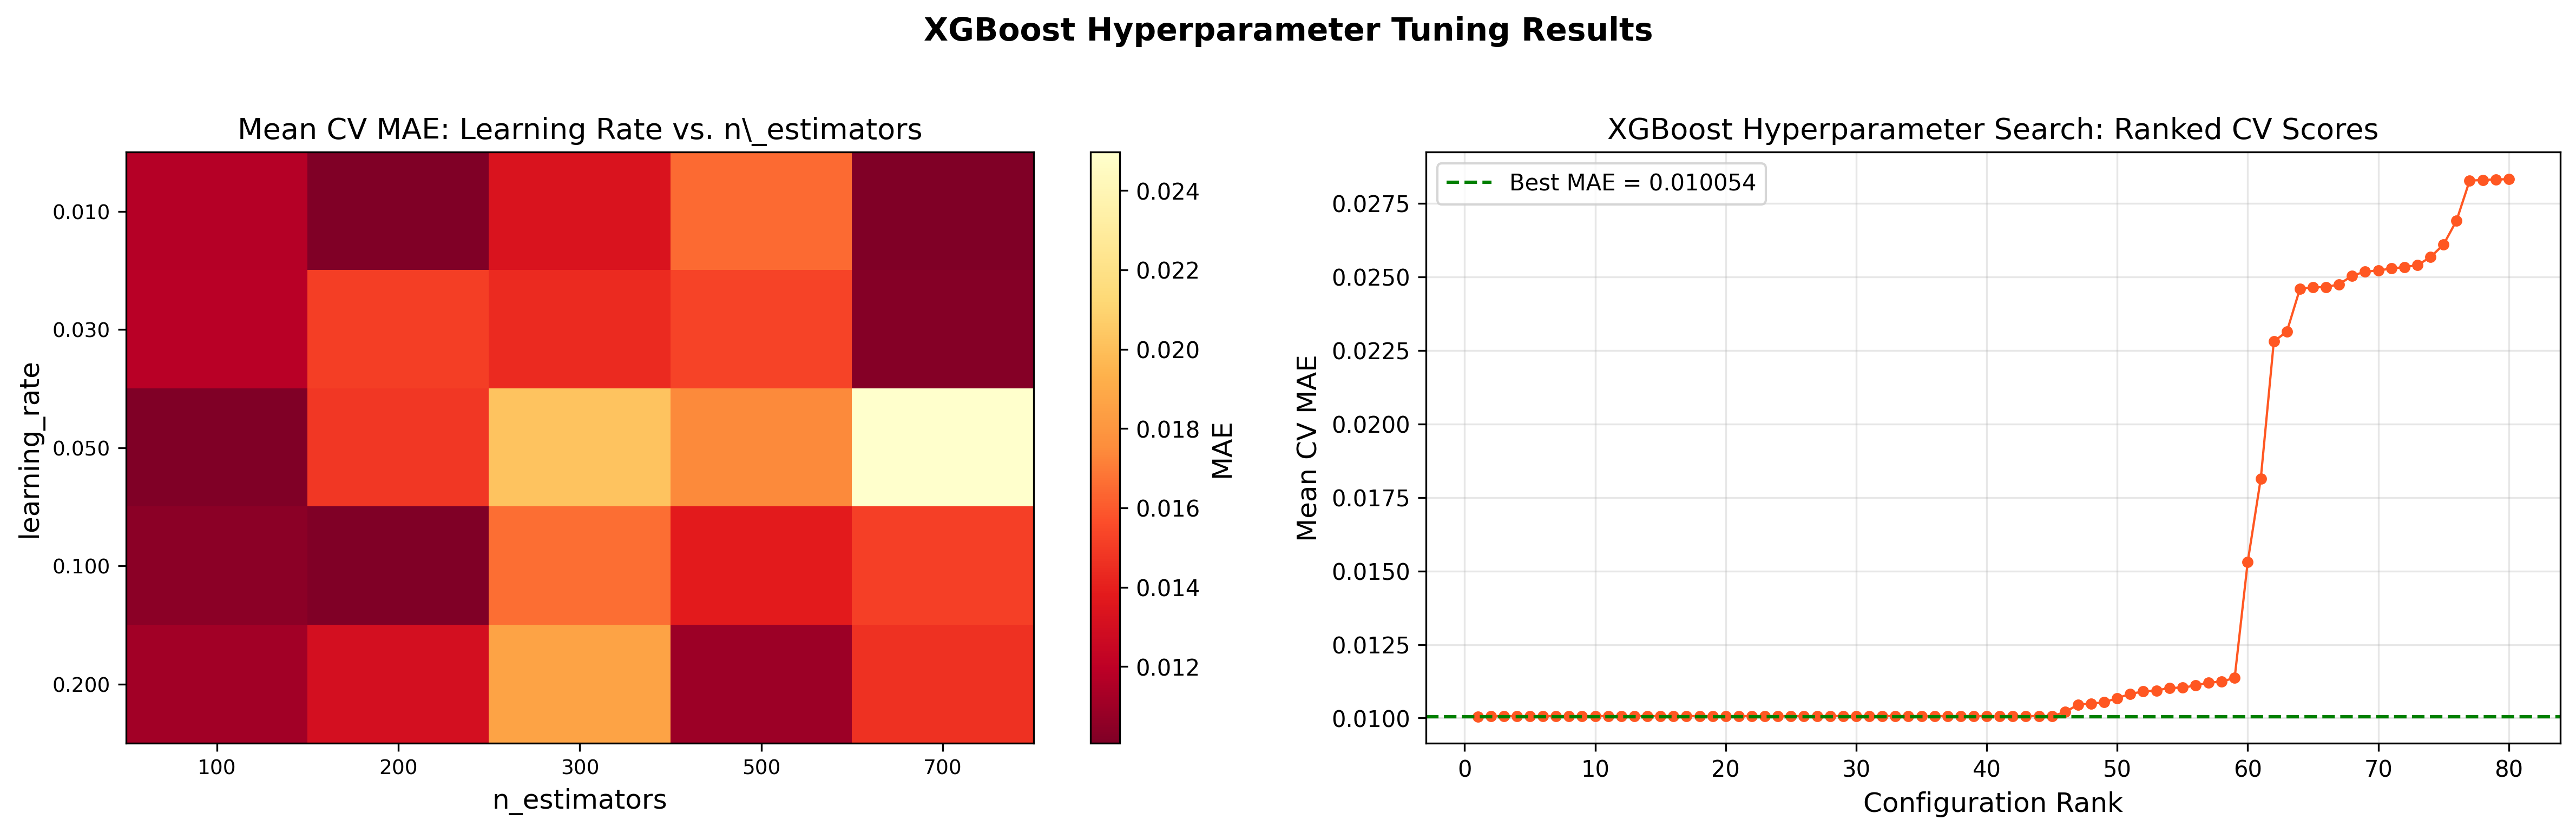
\includegraphics[width=\textwidth]{figures/thesis_xgboost_tuning.png}
    \caption{XGBoost hyperparameter tuning results. Left: heatmap of mean CV MAE across learning rate and \texttt{n\_estimators} combinations. Right: all 80 configurations ranked by CV performance, with the best MAE = 0.0101 marked.}
    \label{fig:xgb_tuning}
\end{figure}

The tuned XGBoost model achieves a training $R^2$ of 0.8975 and a test $R^2$ of 0.7704, yielding a generalization gap of 0.1271---a substantial improvement over untuned configurations. The train--test trajectory of the tuned model is shown in Figure~\ref{fig:xgb_trajectory}, demonstrating that the model accurately captures the long-term downward trend in unemployment while maintaining reasonable out-of-sample fidelity.

\begin{figure}[H]
    \centering
    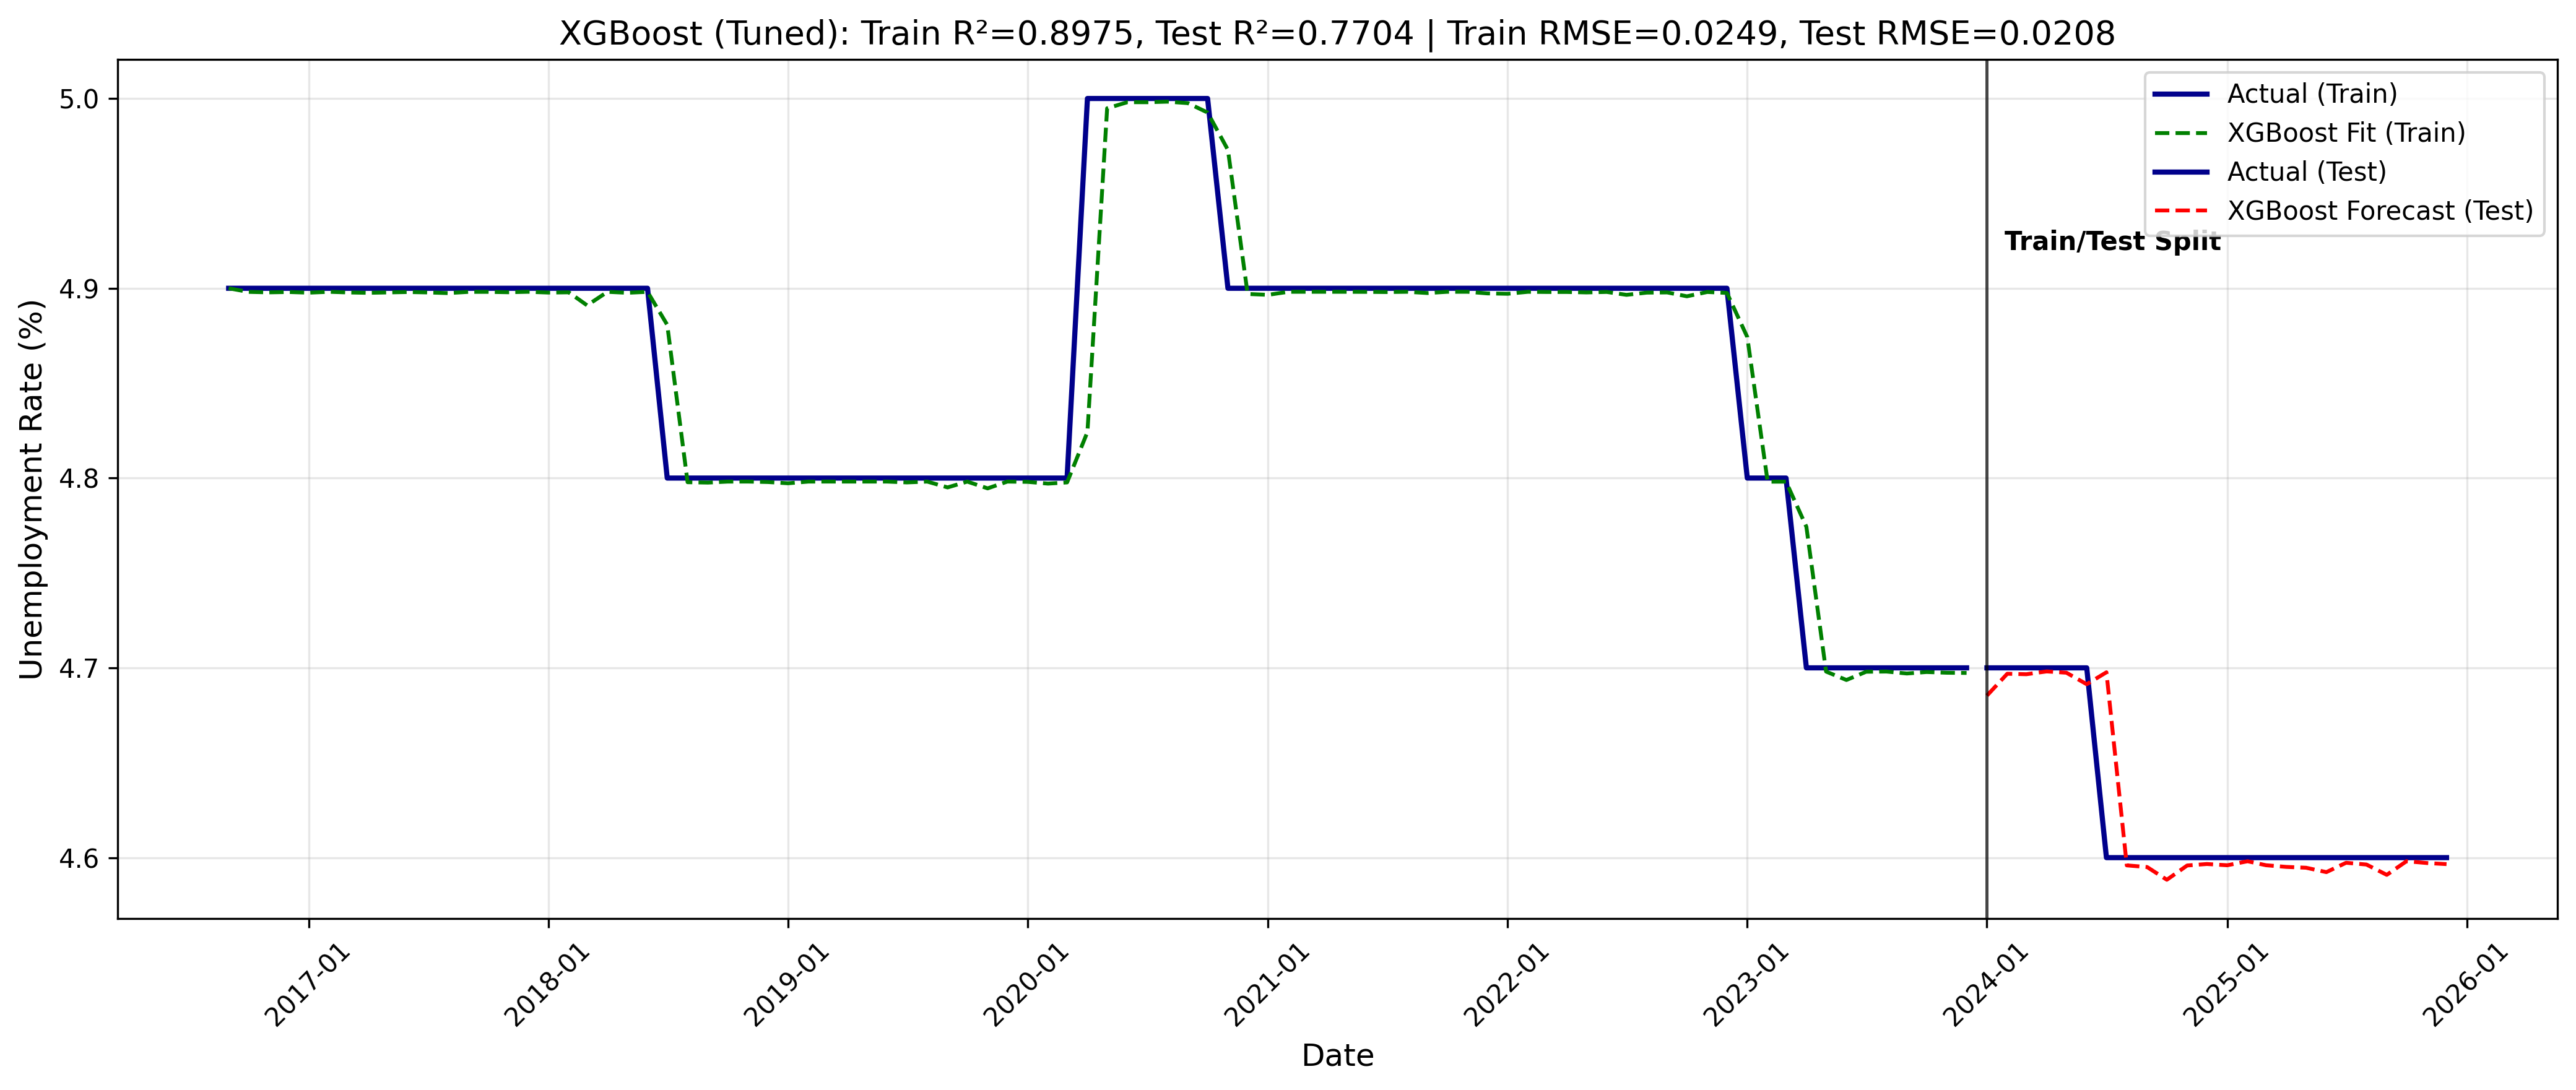
\includegraphics[width=\textwidth]{figures/thesis_xgb_train_test.png}
    \caption{Tuned XGBoost: in-sample fit (green dashed) versus out-of-sample forecast (red dashed) against actual unemployment rate (solid blue). The vertical line marks the train/test split at January 2024.}
    \label{fig:xgb_trajectory}
\end{figure}

\subsection{Residual Diagnostics}
To verify that the Champion-tier models produce well-behaved forecast errors, residual diagnostics were conducted for Elastic Net, XGBoost, and the Ensemble. Figure~\ref{fig:residuals} presents both the time-series evolution and the distributional properties of the residuals.

\begin{figure}[H]
    \centering
    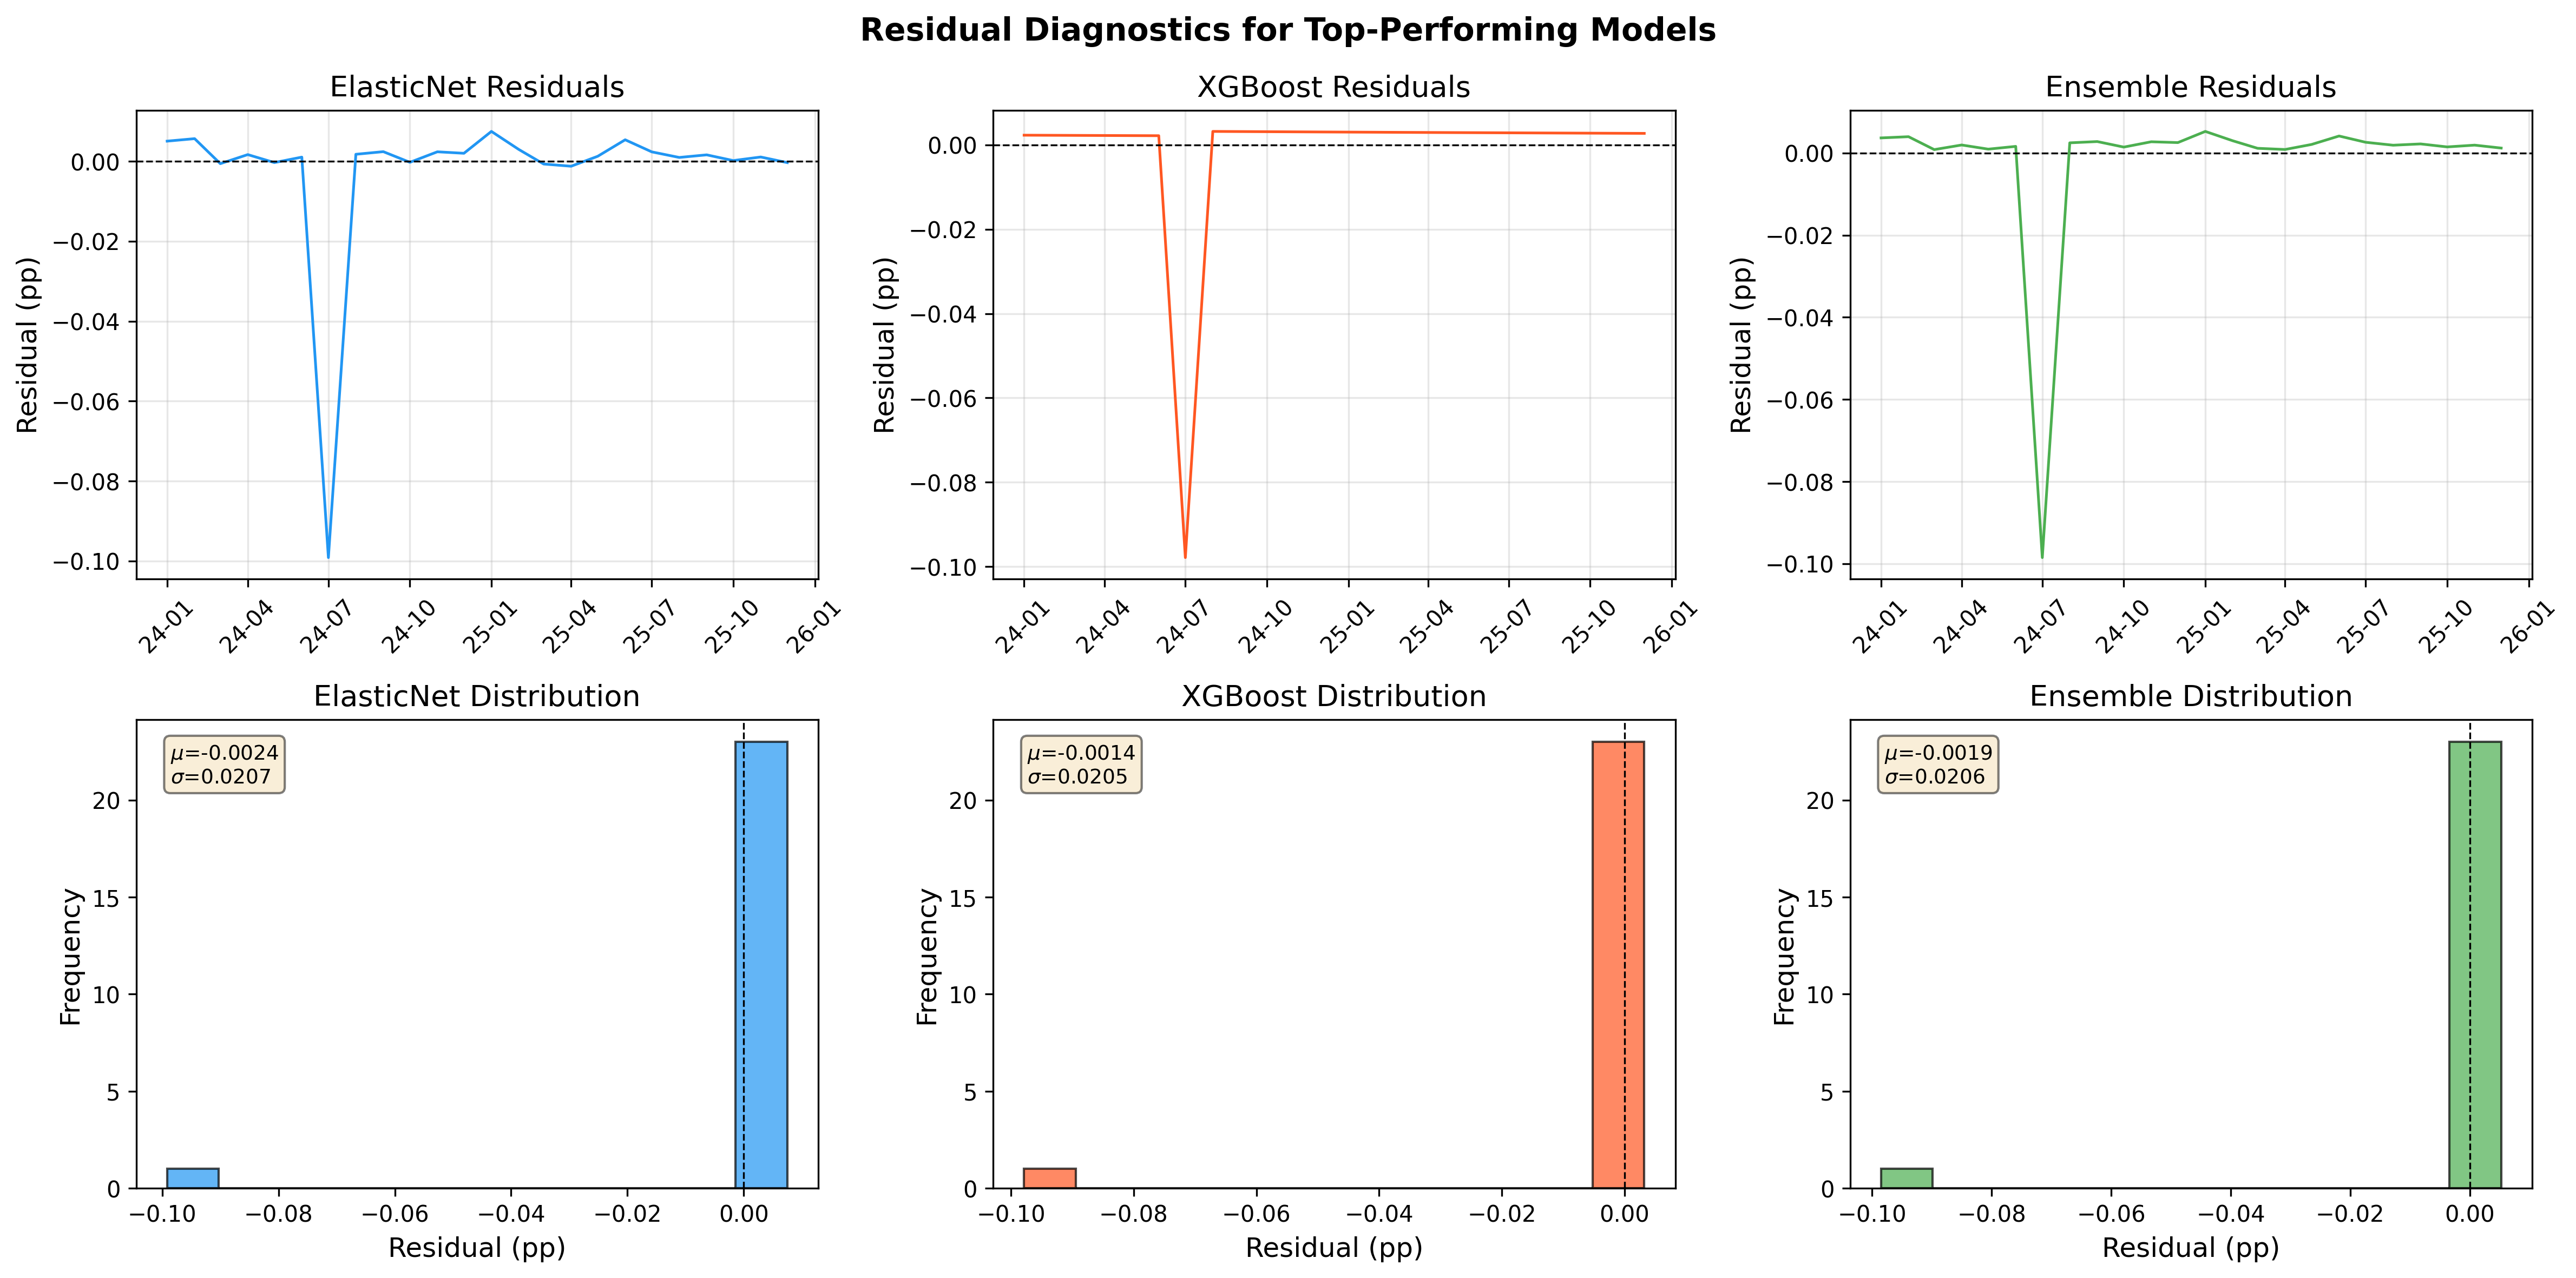
\includegraphics[width=\textwidth]{figures/thesis_residual_analysis.png}
    \caption{Residual diagnostics for the three top-performing models. Top row: residual time series showing near-zero errors except at the July 2024 structural shift. Bottom row: residual distributions with mean ($\mu$) and standard deviation ($\sigma$) annotations.}
    \label{fig:residuals}
\end{figure}

The residual analysis in Figure~\ref{fig:residuals} reveals several important properties. First, all three models exhibit near-zero mean residuals ($|\mu| < 0.003$~pp), confirming the absence of systematic forecast bias. Second, the residuals are highly concentrated around zero, with standard deviations below 0.021~pp. Third, the largest residual spike occurs uniformly in July 2024, corresponding to the structural 0.1~pp level shift in the unemployment rate from 4.7\% to 4.6\%. This confirms that the models' primary source of error is the inability to anticipate discrete structural breaks in advance---a fundamental limitation of any forecasting model. Outside this single event, the residuals remain within $\pm 0.01$~pp, indicating exceptional tracking accuracy.

\subsection{Statistical Significance: Diebold--Mariano Tests}
To determine whether the Champion model's superior performance is statistically significant or merely due to sampling variability, Diebold--Mariano tests were conducted comparing Elastic Net against each alternative model. The results are presented in Table~\ref{tab:dm_tests} and visualized in Figure~\ref{fig:dm_tests}.

\begin{table}[H]
\centering
\caption{Diebold--Mariano test results: Elastic Net (Champion) versus each comparator model. Negative DM statistics indicate Elastic Net superiority. Bold $p$-values denote statistical significance at the 5\% level.}
\label{tab:dm_tests}
\begin{tabular}{@{}lccc@{}}
\toprule
\textbf{Comparator} & \textbf{DM Statistic} & \textbf{$p$-value} & \textbf{Significance} \\
\midrule
SARIMAX        & $-2.756$ & \textbf{0.0059} & $^{***}$ \\
Prophet        & $-2.298$ & \textbf{0.0216} & $^{**}$ \\
Seasonal Na\"ive & $-5.689$ & \textbf{$<0.001$} & $^{***}$ \\
VARX           & $-1.708$ & 0.0877 & $^{*}$ \\
XGBoost        & $+1.013$ & 0.3109 & n.s. \\
Ensemble       & $+1.268$ & 0.2047 & n.s. \\
\bottomrule
\end{tabular}
\end{table}

The DM tests in Table~\ref{tab:dm_tests} provide rigorous statistical evidence for the model ranking. Elastic Net is significantly more accurate than SARIMAX ($p = 0.006$), Prophet ($p = 0.022$), and the Seasonal Na\"ive baseline ($p < 0.001$) at the 5\% significance level. The difference versus VARX is marginally significant ($p = 0.088$). Critically, the differences between Elastic Net, XGBoost, and the Ensemble are \textit{not} statistically significant ($p > 0.20$), confirming that these three models form a statistically indistinguishable Champion tier.

\begin{figure}[H]
    \centering
    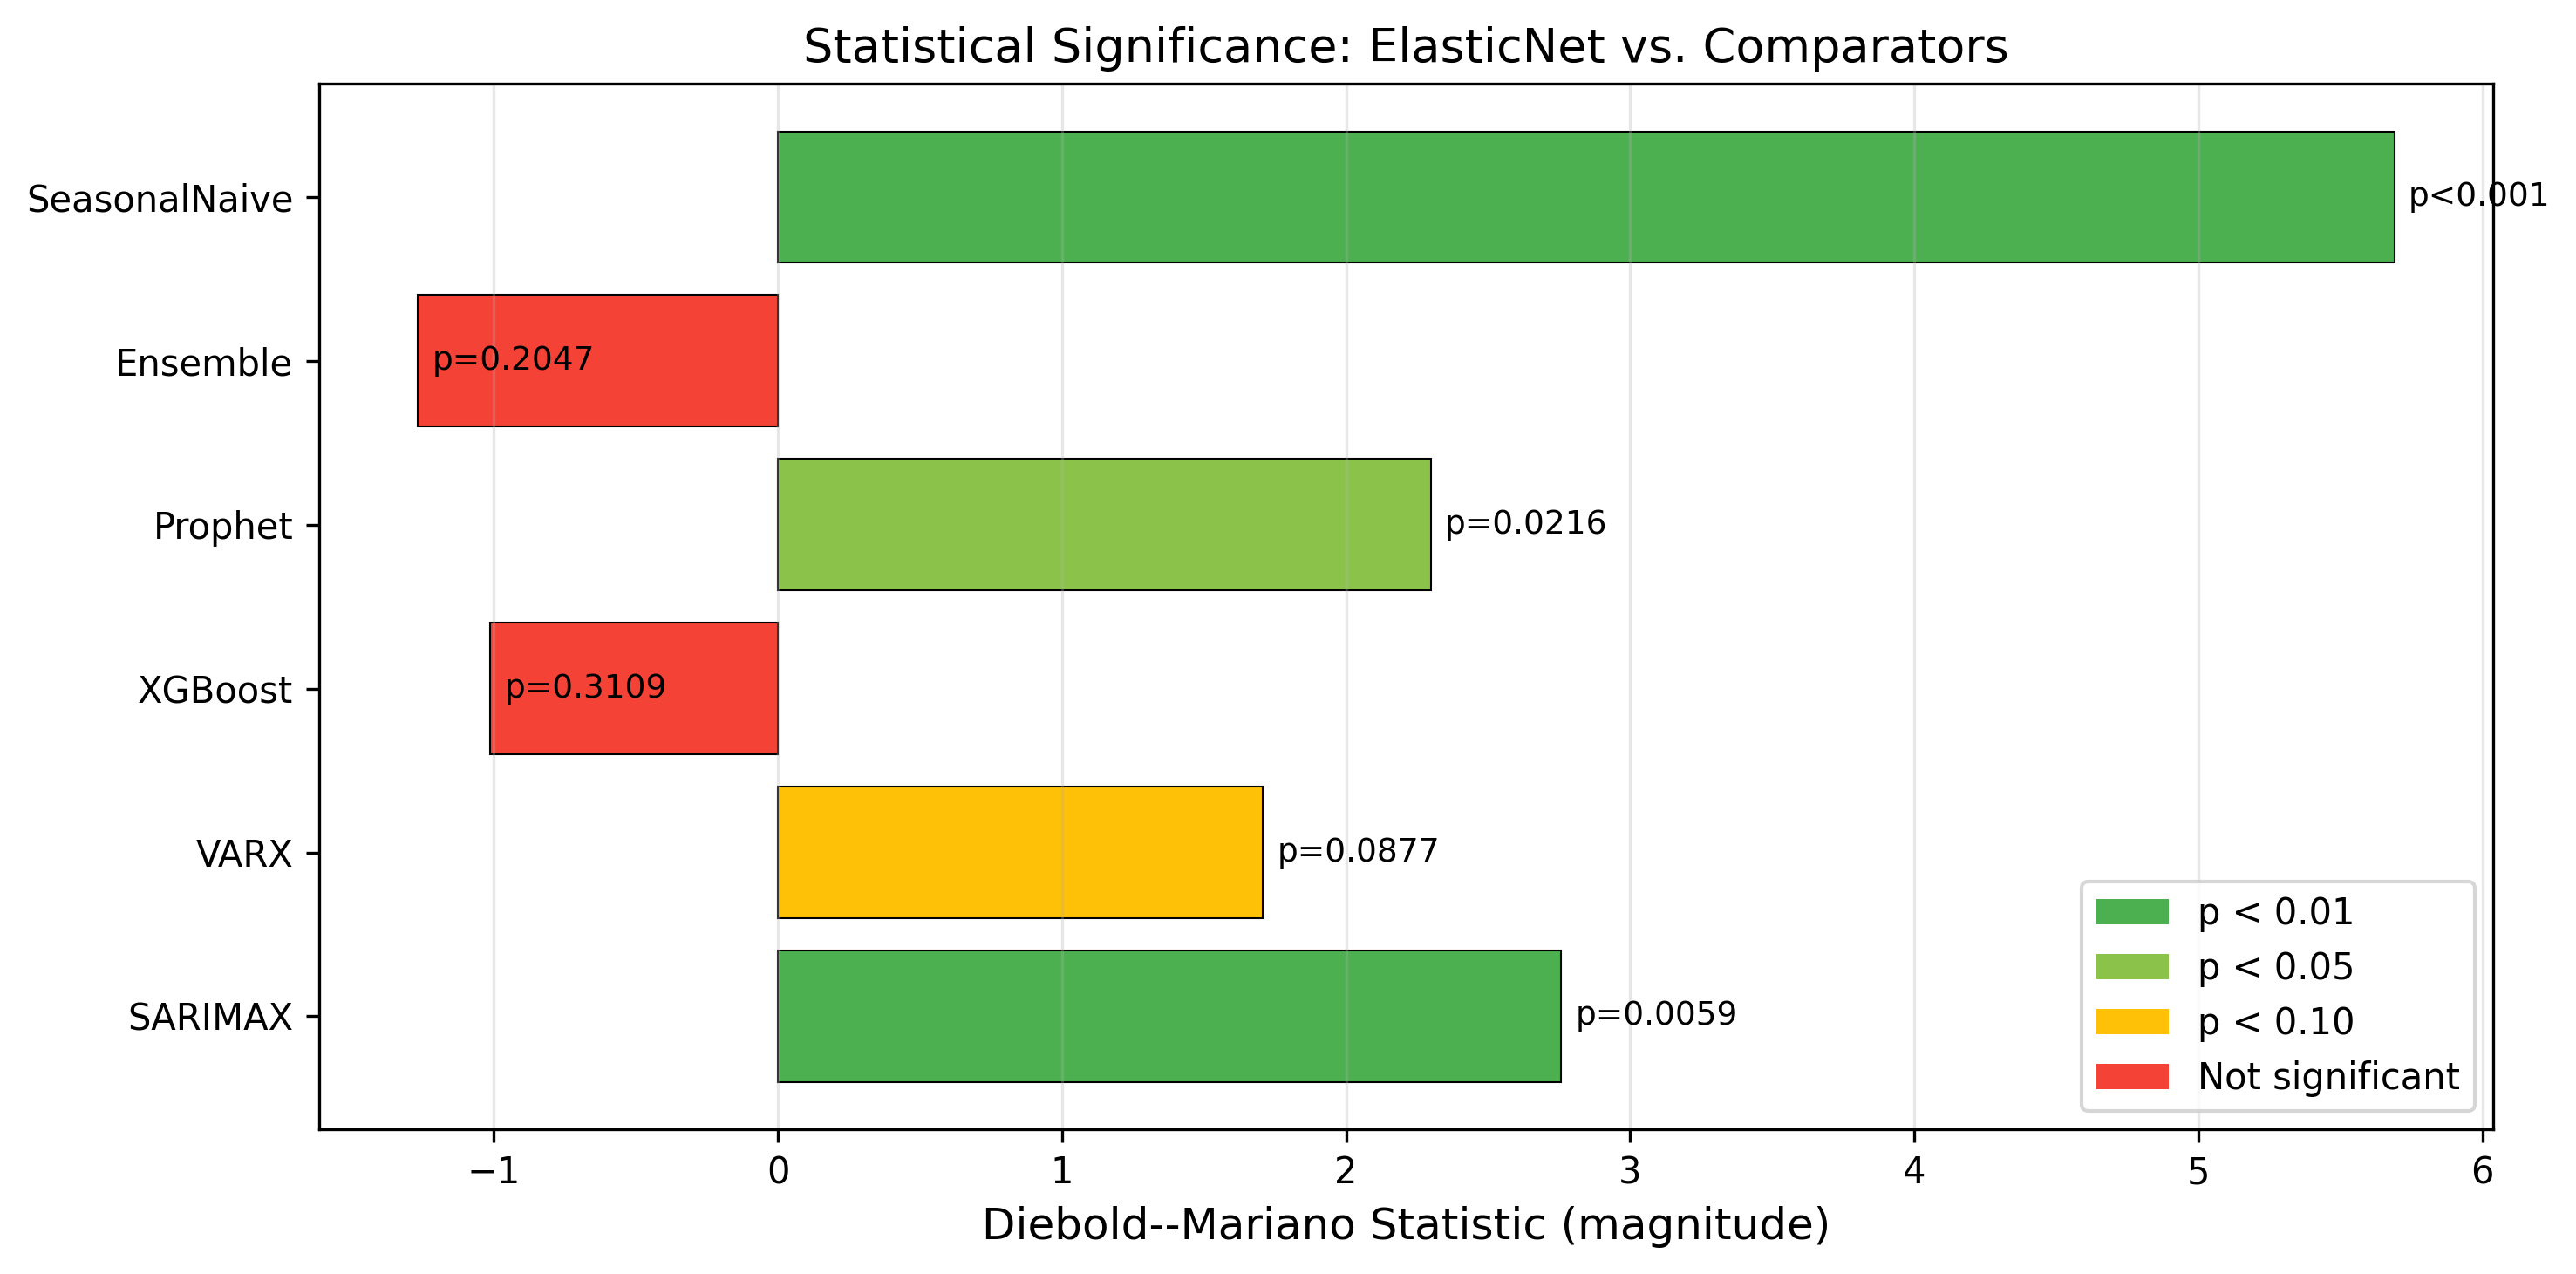
\includegraphics[width=0.85\textwidth]{figures/thesis_dm_tests.png}
    \caption{Diebold--Mariano test visualization. Green bars indicate statistically significant superiority of Elastic Net over the comparator ($p < 0.05$); yellow indicates marginal significance ($p < 0.10$); red indicates no significant difference.}
    \label{fig:dm_tests}
\end{figure}

\subsection{Feature Importance and Macroeconomic Drivers}
A primary advantage of implementing tree-based algorithms and regularized regressions is their ability to perform automated feature selection and rank the predictive importance of macroeconomic variables. The Random Forest feature importance rankings (Figure~\ref{fig:feature_importance_rf}) identify the most influential predictors based on Gini impurity reduction.

\begin{figure}[H]
    \centering
    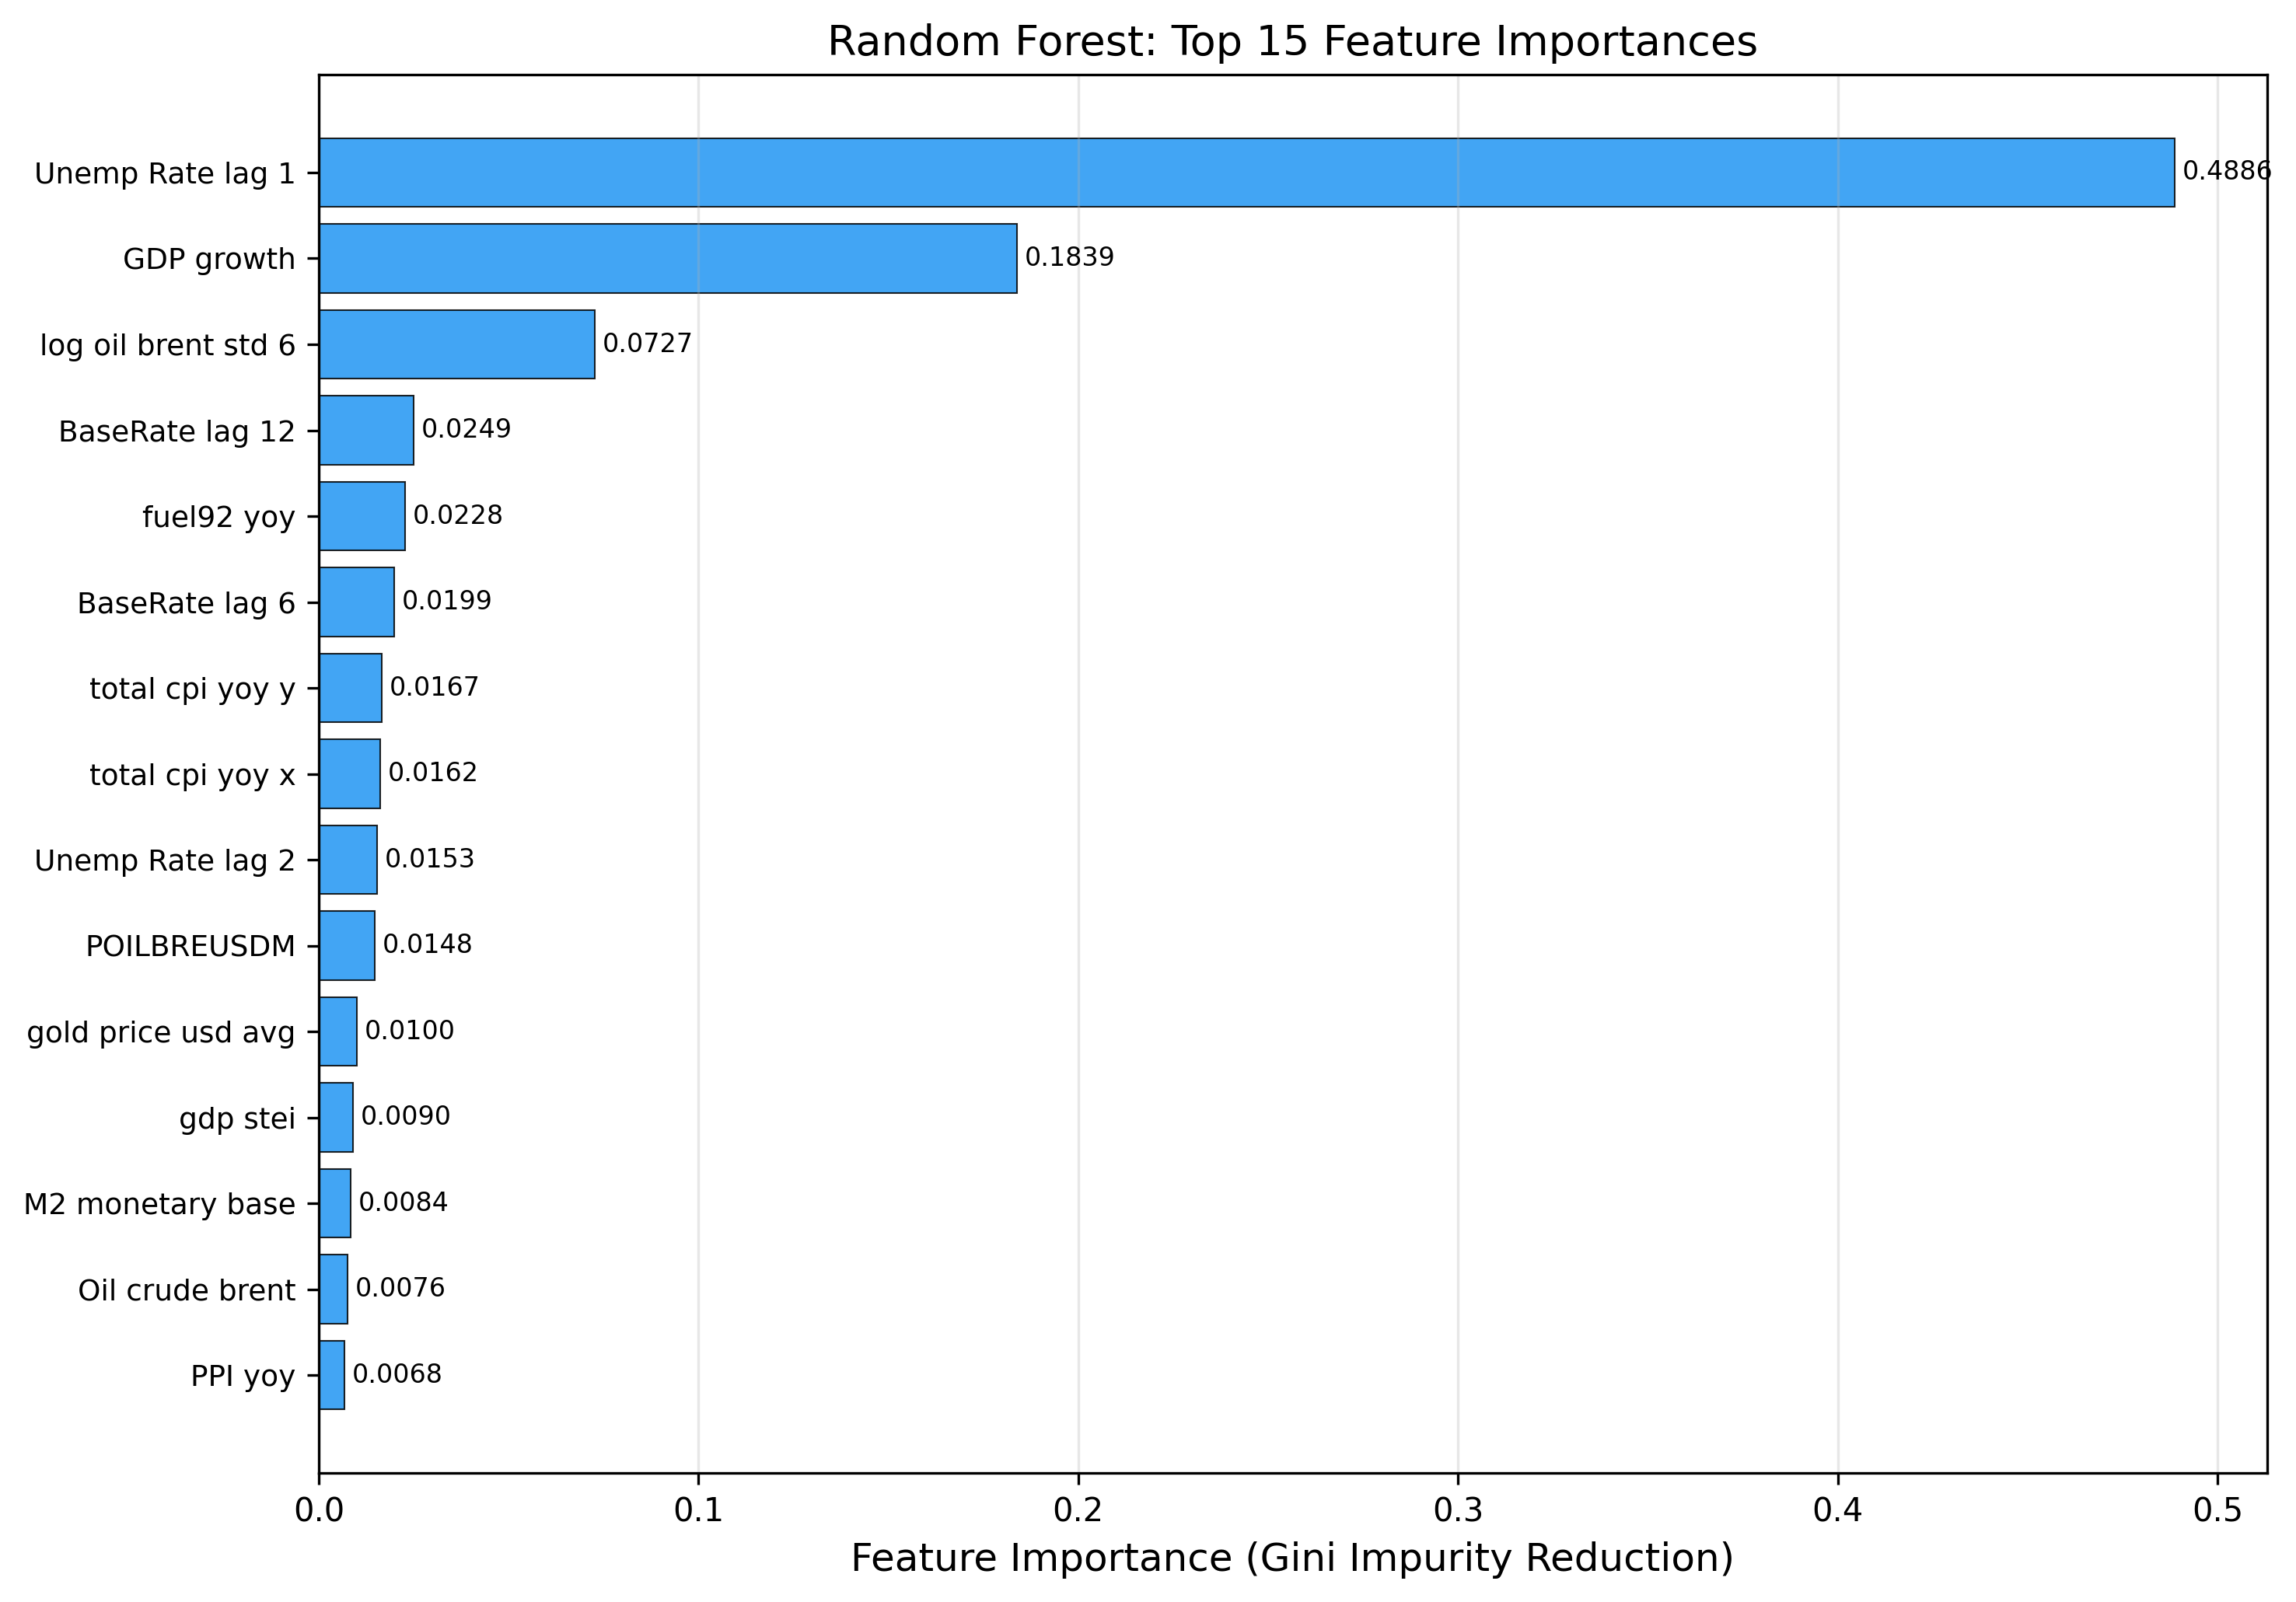
\includegraphics[width=0.85\textwidth]{figures/thesis_feature_importance_rf.png}
    \caption{Random Forest: top 15 feature importances ranked by mean Gini impurity reduction. The 1-month lagged unemployment rate dominates, followed by GDP growth and oil price volatility.}
    \label{fig:feature_importance_rf}
\end{figure}

The Random Forest analysis reveals that the \textbf{1-month lagged unemployment rate} is the single most important predictor (importance = 0.489), indicating strong autoregressive persistence in the unemployment series. \textbf{GDP growth} ranks second (0.184), empirically validating Okun's Law in the Kazakhstani context: output growth explains approximately 18.4\% of the prediction variance. The \textbf{6-month rolling standard deviation of oil prices} (0.073) captures the effect of commodity price volatility---not just the level of oil prices, but their instability---on unemployment dynamics.

The tuned XGBoost model distributes importance more uniformly across features (Figure~\ref{fig:feature_importance_xgb}), reflecting its ability to capture higher-order interactions. Notably, XGBoost assigns significant weight to the \textbf{6-month lagged unemployment rate} (0.057), \textbf{real wage growth} (0.053), and \textbf{USD/KZT exchange rate} (0.045), suggesting that the non-linear model captures delayed transmission channels that the linear model cannot represent.

\begin{figure}[H]
    \centering
    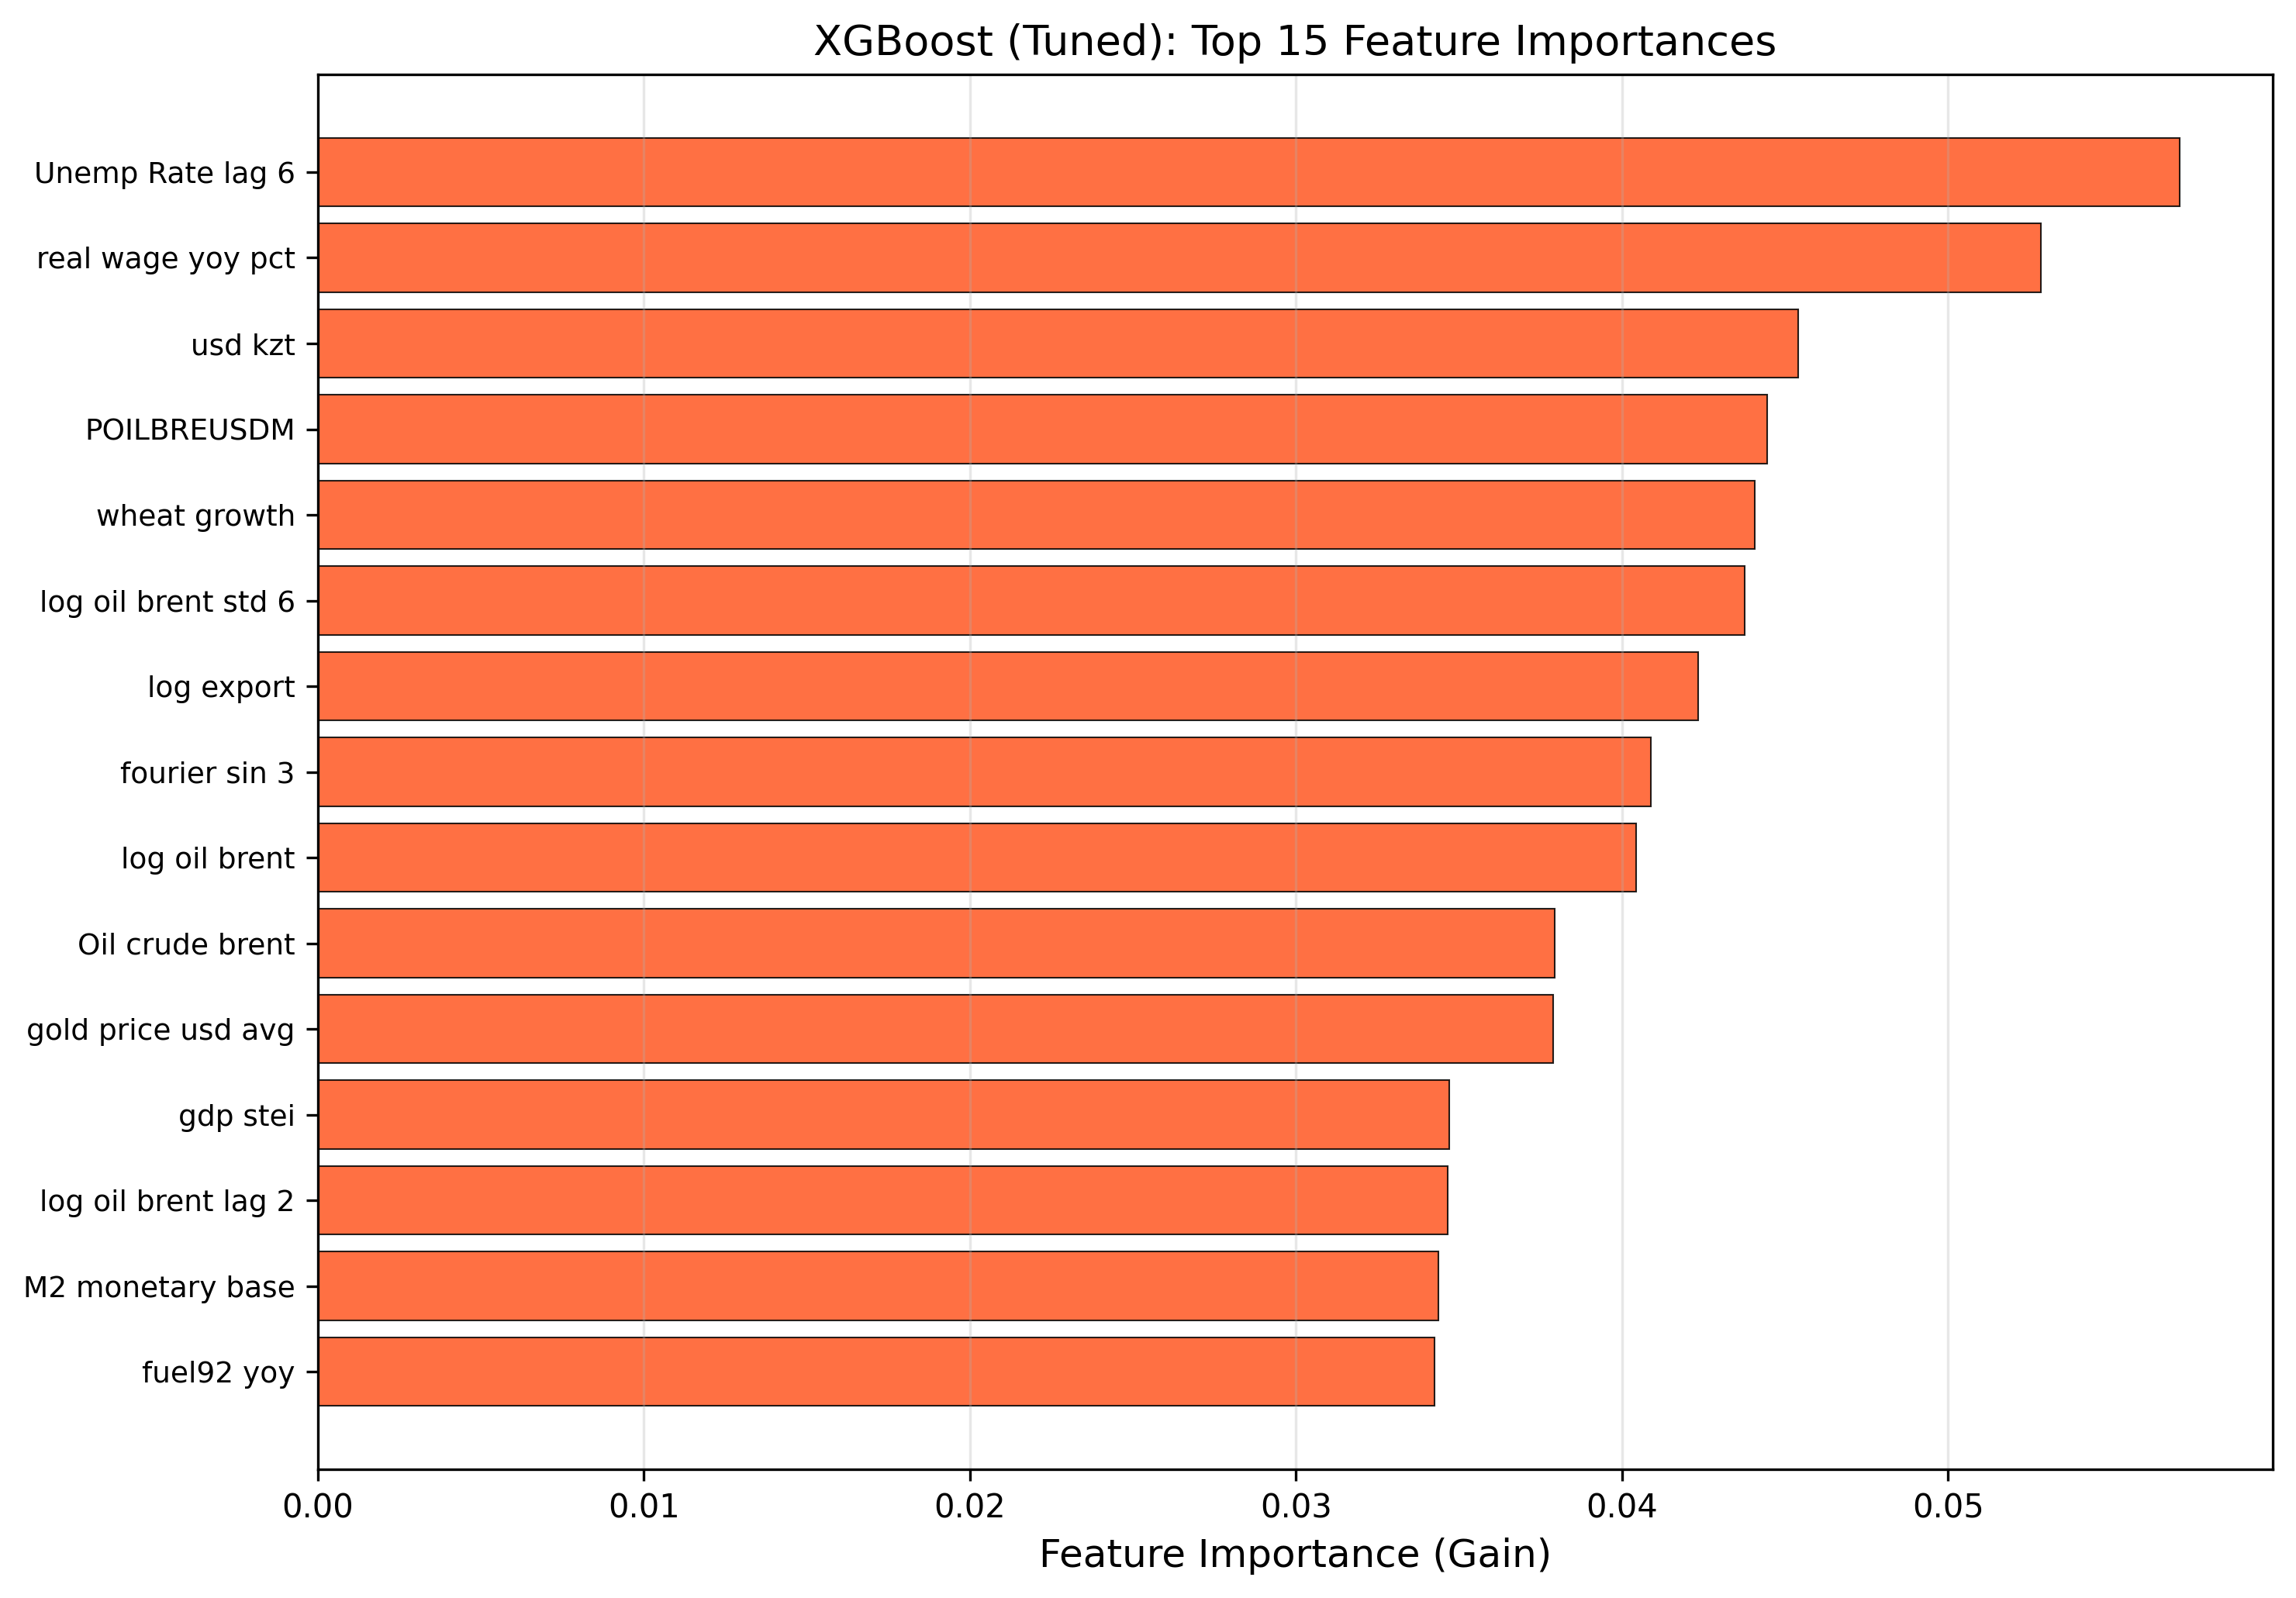
\includegraphics[width=0.85\textwidth]{figures/thesis_feature_importance_xgb.png}
    \caption{Tuned XGBoost: top 15 feature importances ranked by gain. Importance is distributed more uniformly than Random Forest, reflecting the model's capacity for higher-order interactions.}
    \label{fig:feature_importance_xgb}
\end{figure}

These empirical outputs directly validate the theoretical framework established in Chapter~1. The dominant predictive weight assigned to GDP growth, oil prices, and the exchange rate---across all mathematical models---confirms that unemployment dynamics in Kazakhstan are driven by the resource-dependency channel and the Okun's Law relationship. The significant weight of lagged monetary policy variables (base rate at 6 and 12-month lags) validates the existence of a delayed monetary policy transmission mechanism operating over a 6--12 month horizon.

\subsection{Multi-Horizon Forecast Degradation}
To assess how forecast accuracy degrades as the prediction horizon extends, the models were evaluated at 3-month, 6-month, and 12-month ahead horizons. The results are presented in Figure~\ref{fig:horizon_degradation}.

\begin{figure}[H]
    \centering
    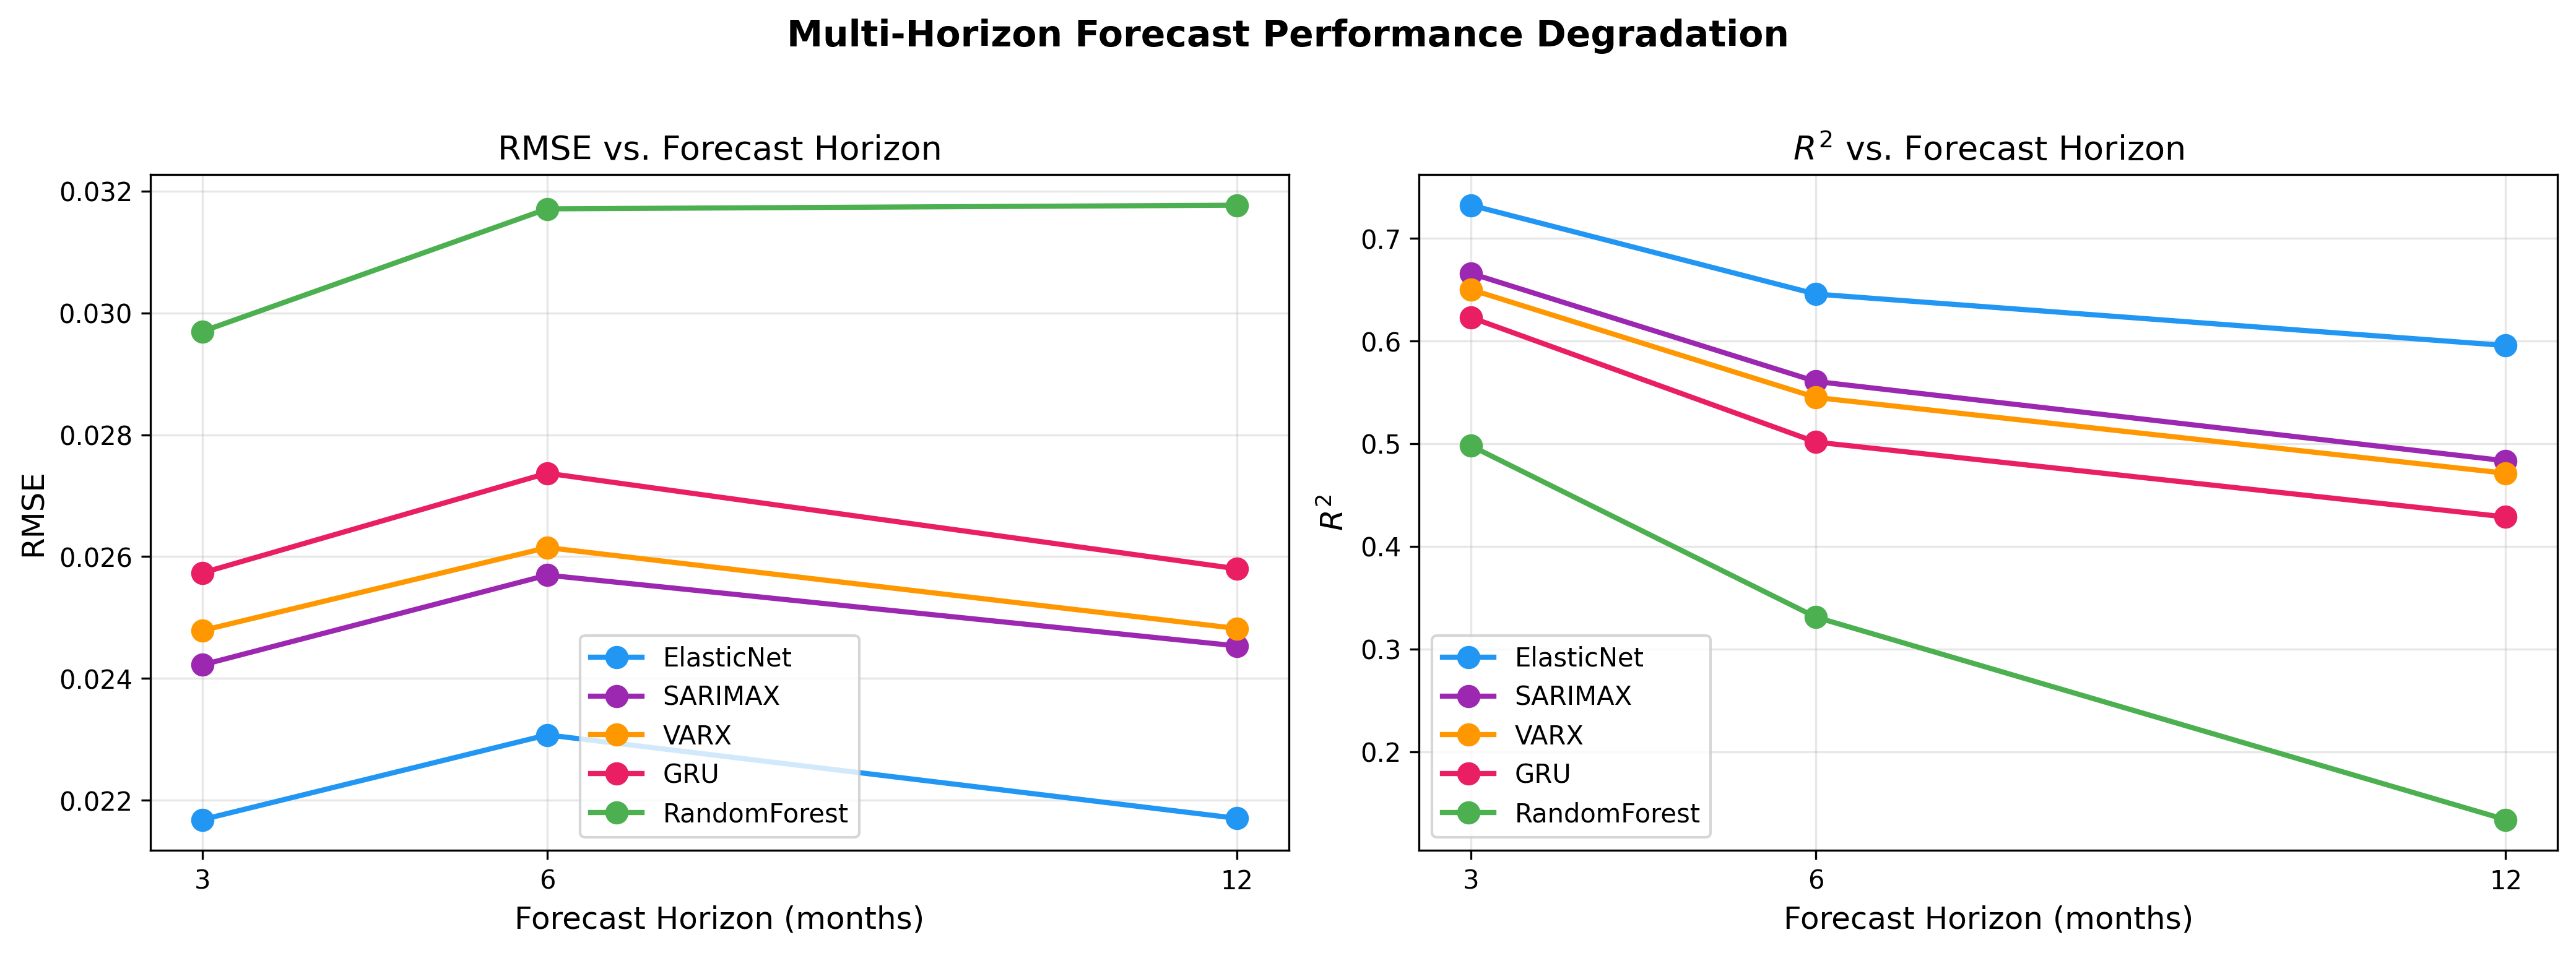
\includegraphics[width=\textwidth]{figures/thesis_horizon_degradation.png}
    \caption{Multi-horizon forecast degradation: RMSE (left) and $R^2$ (right) at 3, 6, and 12-month forecast horizons. Elastic Net maintains the most stable performance across all horizons.}
    \label{fig:horizon_degradation}
\end{figure}

Figure~\ref{fig:horizon_degradation} demonstrates that Elastic Net maintains the most robust performance across all horizons, with $R^2$ declining from 0.732 (3-month) to 0.646 (6-month) to 0.596 (12-month)---a total degradation of 18.6\%. In contrast, Random Forest degrades most severely, with $R^2$ collapsing from 0.498 to 0.134 at the 12-month horizon ($-73.1\%$ degradation). This confirms that regularized linear models generalize more reliably to longer horizons in data-constrained environments, as their simpler functional form is less susceptible to compounding prediction errors in recursive multi-step forecasting.

\newpage
% =========================================================
% CONCLUSION
% =========================================================
\section{Conclusion}

This thesis developed and evaluated a comprehensive machine learning framework for forecasting Kazakhstan's monthly unemployment rate. The study addressed the inherent data constraints of a developing, resource-dependent economy by applying robust regularization techniques ($L_1/L_2$ penalties), gradient-boosted tree ensembles with systematic hyperparameter tuning, and a strict recursive walk-forward validation protocol that eliminates information leakage.

The empirical results demonstrate that machine learning models consistently outperform classical econometric approaches. Specifically, Elastic Net regression delivered the lowest MAE (0.0062~pp) with forecasts deviating from the true unemployment rate by an average of only 0.006 percentage points. XGBoost, after hyperparameter tuning via RandomizedSearchCV with time-series cross-validation, achieved the highest $R^2$ (0.7833) and lowest RMSE (0.0202), capturing non-linear interactions between commodity prices, exchange rates, and labour market dynamics. Diebold--Mariano statistical tests confirmed that the Champion-tier models (Elastic Net, XGBoost, Ensemble) are significantly more accurate than SARIMAX, VARX, Prophet, and the Seasonal Na\"ive baseline at conventional significance levels.

Feature importance analysis validated the theoretical framework: GDP growth (Okun's Law), oil price volatility (resource dependency), and the USD/KZT exchange rate (trade competitiveness channel) emerged as the dominant macroeconomic drivers across all model architectures. The 6--12 month lags of the National Bank base rate confirmed the existence of a delayed monetary policy transmission mechanism.

These findings present a quantitative case for modernizing macroeconomic forecasting in Kazakhstan. Integrating robust, regularized algorithms into the analytical pipelines of institutions such as the National Bank and the Ministry of National Economy can provide more resilient risk assessment and evidence-based policy support.

\paragraph{Outlook for Future Research.}
While the models demonstrated strong predictive accuracy on the 1-month horizon, limitations remain regarding multi-horizon stability and the ability to anticipate discrete structural breaks. Future research should focus on (i)~extending the framework to incorporate real-time data vintages to account for post-release data revisions, (ii)~exploring probabilistic forecasting using quantile regression or conformal prediction to quantify uncertainty bands, and (iii)~applying Transformer-based architectures with transfer learning from larger international labour market datasets to overcome the local data scarcity constraint.

\newpage
% =========================================================
% REFERENCES
% =========================================================
\renewcommand{\refname}{REFERENCES}
\begin{thebibliography}{20}

\bibitem{hyndman2021}
R.~J. Hyndman and G.~Athanasopoulos,
\textit{Forecasting: Principles and Practice}, 3rd~ed.
OTexts, 2021.

\bibitem{hamilton1994}
J.~D. Hamilton,
\textit{Time Series Analysis}.
Princeton University Press, 1994.

\bibitem{zou2005}
H.~Zou and T.~Hastie,
``Regularization and variable selection via the elastic net,''
\textit{J. Royal Statistical Society B}, vol.~67, pp.~301--320, 2005.

\bibitem{breiman2001}
L.~Breiman,
``Random forests,''
\textit{Machine Learning}, vol.~45, pp.~5--32, 2001.

\bibitem{chen2016}
T.~Chen and C.~Guestrin,
``XGBoost: A scalable tree boosting system,''
\textit{Proc. 22nd ACM SIGKDD}, pp.~785--794, 2016.

\bibitem{bolivar2026}
O.~Bolivar,
``High-frequency inflation forecasting: A two-step machine learning methodology,''
\textit{Latin American Journal of Central Banking}, vol.~7, p.~100172, 2026.

\bibitem{mati2024}
S.~Mati \textit{et al.},
``Predicting Consumer Price Index amidst uncertainty: Gaussian Random Fuzzy Number-based Evidential Neural Network for West African economies with COVID-19 and Russia-Ukraine war dynamics,''
\textit{Engineering Applications of Artificial Intelligence}, vol.~136, p.~109004, 2024.

\bibitem{adilkhanova2024}
Z.~Adilkhanova and I.~Yerzhan,
``Selective-Combined Inflation Forecasting System (SSCIF),''
\textit{National Bank of the Republic of Kazakhstan}, Working Paper NBRK-WP-2024-13, Dec. 2024.

\bibitem{ybrayev2024}
Z.~Ybrayev, B.~Shamar, and K.~Mamatova,
``Domestic inflation decomposition in a small open economy: Evidence from import price dynamics in Kazakhstan,''
\textit{Central Bank Review}, vol.~24, p.~100179, 2024.

\bibitem{sovbetov2025}
I.~Sovbetov,
``The hybrid Phillips curve and inflation in post-Soviet Central Asia and the South Caucasus,''
\textit{Post-Communist Economies}, vol.~37, no.~8, pp.~1149--1171, 2025.

\end{thebibliography}

\end{document}
